\chapter[Annexes]{Annexes}

\renewcommand{\contentsname}{Contents}
\localtableofcontents

% \addcontentsline{toc}{chapter}{Annexes}

\chaptermark{Annexes}

%%%%%%%%%%%%%%%%%%%%%%%%%%%%%%%%%%
%%%%%%%%%%%%%%%%%%%%%%%%%%%%%%%%%%
\section{Appendix of Chapter 1}

\subsection{Unbalanced Optimal Transport}

%%%%%%%%%%%%%%%%%%%%%%%%%%%%%%%%%%%%%%%%%%%%%%
\begin{proof}[Proof of \Cref{coro:uot_l2_mm}]
Note that we can write Problem \eqref{uot_l2} as
\begin{align}
    \min_{t \in \bbR^{mn}_{\geq 0}} \langle c, t \rangle + \frac{|| Mt - y ||^2}{2}
\end{align}
where $t = \vect(P), c = \vect(C)$ are the vectorizations of $P, C$, respectively. Here,
\begin{itemize}
    \item[$\bullet$] $M = (\rho_1^{1/2} M_r^T, \rho_2^{1/2} M_c^T, \varepsilon^{1/2} I_{mn})^T \in \bbR^{(m + n + mn) \times (mn)}$.

    \item[$\bullet$] $y = (\rho_1^{1/2} \mu^T, \rho_2^{1/2} \nu^T, \varepsilon^{1/2} \vect(\gamma)^T)^T \in \bbR^{m + n + mn}$.

    \item[$\bullet$] $M_r = \texttt{np.repeat(np.eye(n),m)} \in \bbR^{n \times mn}$.

    \item[$\bullet$] $M_c = [I_m, ..., I_m] = \texttt{np.tile(np.eye(m),n)} \in \bbR^{m \times mn}$.
\end{itemize}
See Appendix A in \citep{Chapel21} for more details of $M_r, M_c$.
Remark that if $A \in \bbR^{m \times n}$ and $B \in \bbR^{m \times p}$, then
\begin{align}
    (A, B) \begin{pmatrix}
        X^T \\
        B^T
    \end{pmatrix}
    = X X^T + B B^T
\end{align}
Following Equation 23 in \citep{Chapel21},  we have
\begin{align}
    t^{(k+1)}_i = t^{(k)}_i \frac{\max( 0, [M^T y]_i - c_i)}{[M^T M t^{(k)}]_i}
\end{align}
Now, $\text{mat}(M^T y) = (\rho_1 \mu) \oplus (\rho_2 \nu) + \varepsilon \gamma$.
Here, matrization is the inverse operation of vectorization. Since,
$M^T M = \rho_1 M_r^T M_r + \rho_2 M_c^T M_c + \varepsilon I_{mn}$, we obtain
$\text{mat}(M^T M t^{(k)}) = (\rho_1 P_{\# 1}^{(k)}) \oplus (\rho_2 P_{\# 2}^{(k)})
+ \varepsilon P^{(k)} $. The result then follows.
\end{proof}
%%%%%%%%%%%%%%%%%%%%%%%%%%%%%%%%%%%%%%%%%%%%%%

%%%%%%%%%%%%%%%%%%%%%%%%%%%%%%%%%%%%%%%%%%%%%%
\begin{proof}[Proof of \Cref{prop:uot_minimizer}]
We follow the same proof technique of Lemma 4 in \citep{Khiem20}.
Given a Bregman divergence $D_{\psi}$, for any $t \in \bbR$ such that $tp \in \text{dom}(\psi)$,
we have
\begin{align}
  D_{\psi}(t p | q)
  &= \psi(tp) - \psi(q) - \langle \nabla \psi(q), tp - q \rangle \\
  &= \psi(tp) - \psi(q) - \Big[
    t \langle \nabla \psi(q), p - q \rangle + (t-1) \langle \nabla \psi(q), q \rangle
  \Big] \\
  &= \psi(tp) - \psi(q) + t \Big[ D_{\psi}(p | q) + \psi(q) - \psi(p) \Big]
  - (t-1) \langle \nabla \psi(q), q \rangle \\
  &= t D_{\psi}(p | q) + \big[ \psi(tp) - t \psi(p) \big]
  + (t-1) \big[ \psi(q) - \langle \nabla \psi(q), q \rangle \big].
\end{align}
Denote $g$ the objective function of Problem \eqref{eq:uot_bregman}. We have,
\begin{align}
  g(tP) &= t g(P) +
  \underbrace{\Big( \sum_{k=1}^2 \rho_k \big[ \varphi_k(tP_{\# k}) - t \varphi_k(P_{\# k}) \big]
  + \varepsilon \big[ \varphi(tP) - t \varphi(P) \big] \Big)}_{A(t)} \\
  &+ (t-1) \underbrace{\Big(
    \sum_{k=1}^2 \rho_k \big[ \varphi_k(\mu_k) - \langle \nabla \varphi_k(\mu_k), \mu_k \rangle \big]
    + \varepsilon \big[ \varphi(\gamma) - \langle \nabla \varphi(\gamma), \gamma \rangle \big]
    \Big)}_{B} \\
    &= t g(P) + A(t) + (t-1) B.
\end{align}
For any minimizer $P^* \in \cC$, denote $\cT^* =\{ t \in \bbR: tP^* \in \cC \}$. Clearly, $\cT^*$ is
not empty since $1 \in \cT^*$. Then $\min_{t \in \cT^*} g(tP^*) = g(P^*)$ and the minimum is
attained when $t=1$. This means $\frac{\partial g(tP^*)}{\partial t} \Big |_{t = 1} = 0$,
or equivalently,
\begin{align}
  g(P^*) &= - B - \frac{\partial A(t)}{\partial t} \bigg|_{t=1} \\
  &= \sum_{k=1}^2 \rho_k \Big[ \langle \nabla \varphi_k(\mu_k), \mu_k \rangle - \varphi_k(\mu_k) \Big]
  + \varepsilon \Big[ \langle \nabla \varphi(\gamma), \gamma \rangle - \varphi(\gamma) \Big] \\
  &+ \sum_{k=1}^2
  \rho_k \Bigg( \varphi_k(P^*_{\# k}) - \frac{\partial \varphi_k(tP^*_{\# k})}{\partial t} \bigg|_{t=1} \Bigg)
  + \varepsilon \Bigg( \varphi(P^*) - \frac{\partial \varphi(tP^*)}{\partial t} \bigg|_{t=1} \Bigg).
\end{align}
The result then follows.
\end{proof}

%%%%%%%%%%%%%%%%%%%%%%%%%%%%%%%%%%%%%%%%%%%%%%
\subsection{Gromov-Wasserstein distance}

%%%%%%%%%%%%%%%%%%%%%%%%%%%%%%%%%%%%%%%%%%%%%%
\begin{corollary}
    The formulations \eqref{GH:zeroth} and \eqref{GH:first} of the Gromov-Hausdorff distance
    are equivalent.
\end{corollary}
\begin{proof}
In the formulation \eqref{GH:first}, by choosing identity mappings (which are clearly isometric embeddings)
$f = \id_X$ and $g = \id_Y$, and $Z = X \cup Y$ equipped with an admissible distance $d$, we have
\begin{equation}
  \gh((X,d_X), (Y,d_Y)) \leq d_{H}^{(Z,d)}(X, Y)
\end{equation}
As this is true for any $d \in \cD(d_X,d_Y)$, we have
$\gh((X,d_X), (Y,d_Y)) \leq \inf_{d} d_{H}^{(X \cup Y, d)}(X, Y)$. For the reverse direction,
given any isometries $f: X \to X'$ and $g: Y \to Y'$ with $X', Y' \subset (Z, d_Z)$
(we call $(X',Y')$ a \textit{metric coupling} \citep{Villani08}), one can define
a distance $d$ on $X \cup Y$ (as shown in Proposition 27.1 in \citep{Villani08}). Then,
\begin{equation}
  \begin{split}
    d_H^{(Z, d_Z)}(f(X), g(Y)) &=
  \max(\sup_{y \in Y} d_Z(g(y), f(X)), \sup_{x \in X} d_Z(f(x), g(Y))) \\
  &= \max(\sup_{y \in Y} d(y, X), \sup_{x \in X} d(x, Y)) \\
  &= d_H^{(X \cup Y, d)}(X, Y) \geq \inf_{d'} d_{H}^{(X \cup Y, d')}(X, Y)
  \end{split}
\end{equation}
We deduce that $\gh((X,d_X), (Y,d_Y)) \geq \inf_{d} d_{H}^{(X \cup Y, d)}(X, Y)$,
thus equality holds.
\end{proof}
%%%%%%%%%%%%%%%%%%%%%%%%%%%%%%%%%%%%%%%%%%%%%%

%%%%%%%%%%%%%%%%%%%%%%%%%%%%%%%%%%%%%%%%%%%%%%
\begin{proof}[Proof of \Cref{lemma:fgw_pgd}]
  Denote $F(P) = \langle C \otimes P, P \rangle + \langle M, P \rangle + \varepsilon \kl(P | \gamma)$.
  Then $\nabla F(P) = C \otimes P + M + \varepsilon \log \frac{P}{\gamma}$.
  The PGD iterate reads: for $\tau > 0$,
  \begin{align}
    P^{(t+1)} = \text{proj}^{\kl}_{U(\mu_x, \mu_y)}
    \left( P^{(t)} \odot e^{-\tau \nabla F(P^{(t)})} \right),
  \end{align}
  where $\text{proj}^{\kl}_{U(\mu_x, \mu_y)}(K) =
  \argmin_{P \in U(\mu_x, \mu_y)} - \varepsilon \langle \log K, P \rangle + \varepsilon H(P)$.
  Denote $\eta = \tau \varepsilon$. We have
  \begin{align}
    \log K &= \log \left( P^{(t)} \odot e^{-\tau \nabla F(P^{(t)})} \right) \\
    &= \log P^{(t)} - \tau (C \otimes P^{(t)} + M)  - \tau \varepsilon \log \frac{P^{(t)}}{\gamma} \\
    &= - \tau (C \otimes P^{(t)} + M) + \log \left( \gamma^{\eta} \odot (P^{(t)})^{1 - \eta} \right).
  \end{align}
  We deduce that
  \begin{align}
    &- \varepsilon \langle \log K, P \rangle + \varepsilon H(P) \\
    &= \eta \langle C \otimes P^{(t)} + M, P \rangle
    - \varepsilon \langle P, \log \left( \gamma^{\eta} \odot (P^{(t)})^{1 - \eta} \right) \rangle
    + \varepsilon H(P) \\
    &= \eta \langle C \otimes P^{(t)} + M, P \rangle +
    \varepsilon \kl \left( P \big | \gamma^{\eta} \odot (P^{(t)})^{1 - \eta} \right)
    - m \left( \gamma^{\eta} \odot (P^{(t)})^{1 - \eta} \right),
  \end{align}
  where $m(Q) = \sum_{i,j} Q_{ij}$ is the mass of measure $Q$. The result then follows.
\end{proof}
%%%%%%%%%%%%%%%%%%%%%%%%%%%%%%%%%%%%%%%%%%%%%%

\subsection{INPUT}
%%%%%%%%%%%%%%%%%%%%%%%%%%%%%%%%%%%%%%%%%%%%%%
\begin{proof}[Proof of \Cref{lemma:convex-smoothness}]
We begin by noticing that $g(\pi) = \kl(\pi | \mu)$ is $1$-strongly convex \wrt the KL divergence.
Indeed, $\nabla g(\pi) = \log \pi - \log \mu$, so for any positive measure $\pi, \gamma$, we have
\begin{align}
    \langle \nabla g(\pi) - \nabla g(\gamma), \pi - \gamma \rangle
    &= \langle
    \log \pi - \log \gamma, \pi - \gamma \rangle.
\end{align}
This means $g$ is $1$-strongly convex \wrt the KL divergence.
To conclude the proof of strong convexity, note that if $f$ is $\sigma$-strongly convex \wrt
some divergence $D$ and $g$ is convex, then the composite function $h = f + g$ is
$\sigma$-strongly convex \wrt $D$. Indeed, for $t \in [0,1]$,
\begin{align}
    h \big( t \pi + (1-t) \gamma \big)
    &= f \big( t \pi + (1-t) \gamma \big) + g \big( t \pi + (1-t) \gamma \big) \\
    &\leq t f(\pi) + (1 - t) f(\gamma) - \sigma \frac{t (1 - t)}{2} D(\pi, \gamma)
    + t g(\pi) + (1 - t) g(\gamma) \\
    &= t h(\pi) + (1 - t) h(\gamma) - \sigma \frac{t (1 - t)}{2} D(\pi, \gamma).
\end{align}
Regarding the relative smoothness, denote $h(\pi) = \kl(\pi_{\#1} | \alpha)$,
then $(\nabla h(\pi))_{ij} = \log (\pi_{\#1})_i - \log \alpha_i$, for every $j$. So,
\begin{equation}
    \begin{split}
        \langle \nabla h(\pi) - \nabla h(\gamma), \pi - \gamma \rangle
    &= \langle
    \log \pi_{\# 1} - \log \gamma_{\# 1}, \pi_{\# 1} - \gamma_{\# 1} \rangle\\
    &= \kl(\pi_{\# 1} | \gamma_{\# 1}) + \kl(\gamma_{\# 1} | \pi_{\# 1}) \\
    &\leq \kl(\pi | \gamma) + \kl(\gamma | \pi) \\
    &= \langle \log \pi - \log \gamma, \pi - \gamma \rangle
    \end{split}
\end{equation}
where the last inequality is due to the data pre-processing inequality.
This means that $h$ is $1$-relatively smooth \wrt the KL divergence.
We conclude that $F$ is $(\lambda_1 + \lambda_2 + \varepsilon)$-relatively smooth.
\end{proof}
%%%%%%%%%%%%%%%%%%%%%%%%%%%%%%%%%%%%%%%%%%%%%%

%%%%%%%%%%%%%%%%%%%%%%%%%%%%%%%%%%%%%%%%%%%%%%
\begin{proof}[Proof of \Cref{prop:convergence-exact-sppa}]
We adapt the proof of Theorem 3.1 in \citep{Lu18}.
First, recall the 4-points identity of Bregman divergence.
\begin{lemma}[Four-point lemma]
    \label{lemma:four-points}
    For any $x, y, z, t \in \text{dom}(\varphi)$, we have
    \begin{equation}
    D_{\varphi}(z, y) - D_{\varphi}(z,x) + D_{\varphi}(t, x) - D_{\varphi}(t, y)
    = \langle \nabla \varphi(x) - \nabla \varphi(y), z - t \rangle.
    \end{equation}
    As a consequence, by taking $y = t$, we obtain the three-point lemma
    \begin{equation}
    D_{\varphi}(z, y) + D_{\varphi}(y, x) - D_{\varphi}(z, x)
    = \langle \nabla \varphi(x) - \nabla \varphi(y), z - y \rangle.
    \end{equation}
\end{lemma}

%%%%%%%%%%%%%%%%%%%%%%%%%%%%%%%%%%%%%%%%%%%%%%%%%%%
\begin{lemma}[Adapted from Lemma 3.2 in \citep{Chen93}]
    \label{lemma:bregman-minimizer-property}
    Suppose $f$ is a $l$-strongly convex, proper differentiable function whose domain is a closed set
    $C$. Let $ x^{(t+1)} = \argmin_{x \in C} f(x) + D_{\varphi}\left(x, x^{(t)} \right)$.
    Then, for any $x \in C$, we have
    \begin{align}
        f(x^{(t+1)}) + (l+1) D_{\varphi}(x, x^{(t+1)}) + D_{\varphi} (x^{(t+1)}, x^{(t)})
        \leq f(x) + D_{\varphi} (x, x^{(t)}).
    \end{align}
    Moreover, if $f$ is also $L$-smooth, then
    \begin{align}
            f(x^{(t+1)}) + (L+1) D_{\varphi}(x, x^{(t+1)}) + D_{\varphi} (x^{(t+1)}, x^{(t)})
            \geq f(x) + D_{\varphi} (x, x^{(t)}).
        \end{align}
\end{lemma}
\begin{proof}[Proof of \Cref{lemma:bregman-minimizer-property}]
    From the optimality of $x^{(t+1)}$, we have
    $\nabla \varphi(x^{(t+1)}) - \nabla \varphi(x^{(t)}) + \nabla f(x^{(t+1)}) = 0$.
    By three-point lemma, for every $x \in C$,
    \begin{align}
        D_{\varphi}(x, x^{(t+1)}) + D_{\varphi} (x^{(t+1)}, x^{(t)}) - D_{\varphi} (x, x^{(t)}) &= \langle \nabla \varphi(x^{(t)}) - \nabla \varphi(x^{(t+1)}), x - x^{(t+1)} \rangle \\
        &= \langle \nabla f(x^{(t+1)}), x - x^{(t+1)} \rangle.
    \end{align}
    As $f$ is $l-$strongly convex and differentiable, we have
    \begin{align}
        f(x) &\geq f(x^{(t+1)}) + \langle \nabla f(x^{(t+1)}), x -
                x^{(t+1)} \rangle  + l D_{\varphi}(x, x^{(t+1)})\\
        &=         f(x^{(t+1)}) + (l+1) D_{\varphi}(x, x^{(t+1)})
        + D_{\varphi} (x^{(t+1)}, x^{(t)}) - D_{\varphi} (x, x^{(t)}).
    \end{align}
    Similarly, if $f$ is $L$-relatively smooth, then
    \begin{align}
        f(x) &\leq f(x^{(t+1)}) + \langle \nabla f(x^{(t+1)}), x -
                x^{(t+1)} \rangle  + L D_{\varphi}(x, x^{(t+1)})\\
        &=         f(x^{(t+1)}) + (L+1) D_{\varphi}(x, x^{(t+1)})
        + D_{\varphi} (x^{(t+1)}, x^{(t)}) - D_{\varphi} (x, x^{(t)}).
    \end{align}
    The result then follows.
\end{proof}
%%%%%%%%%%%%%%%%%%%%%%%%%%%%%

%%%%%%%%%%%%%%%%%%%%%%%%%%%%%
\begin{lemma}
    \label{lemma:bound_seq}
    If $(y_t)_t$ is a nonnegative decreasing sequence, $(x_t)_t$ is a nonnegative sequence and
    $a, b > 0$ such that $y_t \leq a x_{t-1} - b x_t$, then
    $y_t \leq \frac{b-a}{\left( \frac{b}{a} \right)^t - 1} x_0$.
\end{lemma}
\begin{proof}[Proof of \Cref{lemma:bound_seq}]
We have that $\frac{y_t}{b} \leq \frac{a}{b} x_{t-1} - x_t$. So,
$\left( \frac{a}{b} \right)^i \frac{y_{t-i}}{b} \leq
\left(\frac{a}{b} \right)^{i+1} x_{t-i-1} - \left( \frac{a}{b} \right)^i x_{t-i}$.
Computing the telescopic sum, we have
\begin{align}
    \left( \frac{a}{b} \right)^t x_0 - x_t &\geq
    \sum_{i=0}^{t-1} \left( \frac{a}{b} \right)^i \frac{y_{t-i}}{b}
    \geq \frac{y_t}{b} \frac{\left( \frac{a}{b} \right)^t - 1}{\frac{a}{b} - 1}
    = y_t \frac{\left( \frac{a}{b} \right)^t - 1}{a - b}.
\end{align}
Since $x_t \geq 0$, we deduce that
$y_t \leq \frac{b-a}{\left( \frac{b}{a} \right)^t - 1} x_0$.
\end{proof}
%%%%%%%%%%%%%%%%%%%%%%%%%%%%%

%%%%%%%%%%%%%%%%%%%%%%%%%%%%%
\begin{lemma}
\label{lemma:bppa_conv}
    Let $F$ be a differentiable function. Suppose that $F$ is $l-$strongly convex and $L-$ smooth,
    where $L > l \geq 0$. Given a learning rate $l \leq \eta \leq L$,
    define $x^{(t+1)} = \argmin F(x) + \eta D_{\varphi}(x, x^{(t)})$.
    Then, for any initialization $x^{(0)}$, we have
    \begin{align}
        F(x^{(t)}) - F(x^*) \leq \frac{l}{\left( 1 + \frac{Ll }{\eta (L - l)} \right)^t - 1}
        D_{\varphi}(x^*, x^{(0)}).
\end{align}
\end{lemma}
%%%%%%%%%%%%%%%%%%%%%%%%%%%%%
\begin{proof}[Proof of \Cref{lemma:bppa_conv}]
By applying \Cref{lemma:bregman-minimizer-property} with $f = \frac{F}{\eta}$,
which is $\frac{l}{\eta}-$strongly convex, we obtain that
\begin{equation}
    D_{\varphi}(x^{(t+1)}, x^{(t)}) \leq D_{\varphi}(x, x^{(t)})
    - \left( \frac{l}{\eta} + 1 \right) D_{\varphi}(x, x^{(t+1)})
    - \frac{F(x^{(t+1)}) - F(x)}{\eta}.
\end{equation}
In particular, by choosing $x = x^{(t)}$, we have
\begin{equation}
    F(x^{(t+1)}) - F(x^{(t)}) \leq - \eta \left[ \left(\frac{l}{\eta} + 1 \right)
    D_{\varphi}(x^{(t)}, x^{(t+1)}) + D_{\varphi}(x^{(t+1)}, x^{(t)}) \right] \leq 0.
\end{equation}
This means $\big(F(x^{(t)}) \big)_t$ is a (nonnegative) decreasing sequence.
Now, for every $x \in C$ and $l \leq \eta \leq L$,
\begin{align}
    &F(x^{(t+1)}) \\
    &\leq F(x^{(t)}) + \langle \nabla F(x^{(t)}), x^{(t+1)} - x^{(t)} \rangle
    + L D_{\varphi}(x^{(t+1)}, x^{(t)}) \\
    &\leq F(x^{(t)}) + \langle \nabla F(x^{(t)}), x - x^{(t)} \rangle
    + \eta D_{\varphi}(x, x^{(t)}) - \eta D(x, x^{(t+1)})
    + (L - \eta) D_{\varphi}(x^{(t+1)}, x^{(t)}) \\
    &\leq F(x) + (\eta - l) D_{\varphi}(x, x^{(t)})
    - \eta D(x, x^{(t+1)}) + (L - \eta) D_{\varphi}(x^{(t+1)}, x^{(t)}) \\
    &\leq F(x) + (\eta - l) D_{\varphi}(x, x^{(t)}) - \eta D(x, x^{(t+1)}) \\
    &+ (L - \eta) \left[ D_{\varphi}(x, x^{(t)})
    - \left( \frac{l}{\eta} + 1 \right) D_{\varphi}(x, x^{(t+1)})
    - \frac{F(x^{(t+1)}) - F(x)}{\eta} \right] \\
    &= F(x) + (L - l) D_{\varphi}(x, x^{(t)})
    - \left[ L + \frac{l}{\eta}(L - \eta) \right] D_{\varphi}(x, x^{(t+1)})
    - \frac{L - \eta}{\eta} \big[ F(x^{(t+1)}) - F(x) \big],
\end{align}
where the first and third inequalities follow from the strong convexity and
relative smoothness of $F$, respectively. The second one follows by applying
\Cref{lemma:bregman-minimizer-property} with
$f = \frac{1}{\eta} \langle \nabla F(x^{(t)}), \cdot - x^{(t)} \rangle$
(which is $0$-strongly convex). By rearranging the terms, we obtain
\begin{align}
    F(x^{(t+1)}) - F(x) \leq \frac{\eta(L-l)}{L} D_{\varphi}(x, x^{(t)})
    - \left[ l + \frac{\eta (L - l)}{L} \right] D_{\varphi}(x, x^{(t+1)}).
\end{align}
By applying \Cref{lemma:bound_seq} and choosing $x = x^*$, we deduce that
\begin{align}
    F(x^{(t)}) - F(x^*) \leq \frac{l}{\left( 1 + \frac{Ll }{\eta (L - l)} \right)^t - 1}
    D_{\varphi}(x, x^{(0)}).
\end{align}
The result then follows.
\end{proof}
Now, \Cref{prop:convergence-exact-sppa} follows immediately from
\Cref{lemma:bppa_conv,lemma:convex-smoothness}.
\end{proof}
%%%%%%%%%%%%%%%%%%%%%%%%%%%%%%%%%%%%%%%%%%%%%%

%%%%%%%%%%%%%%%%%%%%%%%%%%%%%%%%%%%%%%%%%%%%%%
\section{Appendix of Chapter 2}

\subsection{Discrete Co-Optimal Transport}

One can rewrite the problem as
\begin{align}
  \vect{P}^T C^x \otimes C^y \vect{P}
\end{align}
\begin{proposition}
  (Theorem 1 in \citep{Maron18}) Denote
\begin{equation}
    \text{lin(DS)} = \{X \in \bbR^{m \times n}: X 1_n = 0, X^T 1_m = 0 \}
\end{equation}
the linear part of the affine-hull of the doubly-stochastic matrices. If the matrices $A \in \bbR^{m \times m}$ and
  $B \in \bbR^{n \times n}$ are both conditionally negative (or positive) semi-definite, then $\text{vec}(X)^T (B \otimes A) \text{vec}(X) \geq 0$, for every $X \in \text{lin(DS)}$.
\end{proposition}
\begin{proof}
    By lemma above, it's enough to show for any $X = u v^T$, where $u \in 1^{\perp}_m$
    and $v \in 1^{\perp}_n$. In this case, as
    $(U \otimes V)^T (A \otimes B) (U \otimes V) = (U^T A U) \otimes (V^T B V)$, we have
    $\text{vec}(u v^T)^T (B \otimes A) \text{vec}(u v^T) = (u^T A u) (v^T B v) \geq 0$.
\end{proof}

First, let us define three following reshaping operations.
\begin{itemize}
  \item[$\bullet$] Vectorization: concatenates rows of a matrix into a vector.
  \begin{equation*}
    \vect: \bbR^{m \times n} \to \bbR^{m n},
  \end{equation*}
  where each element $A_{i,j}$ of the matrix $A \in \bbR^{m \times n}$ is
  mapped to a unique element $b_{(i-1)n + j}$ of the vector
  $b \in \bbR^{m n}$, with $A_{i,j} = b_{(i-1)n + j}$, for $i = 1, ..., m$ and $j = 1, ...,n$.
  Conversely, each element $b_k$ is mapped to a unique element $A_{k // n, n - k \% n}$,
  for every $k = 1, ..., mn$. Here, $k // n$ and $k \% n$ are the quotient and
  the remainder of the division of $k$ by $n$,
  respectively, \ie, if $k = q n + r$, with $0 \leq r < n$, then $k // n = q$ and $k \% n = r$.

  \item[$\bullet$] Matrization: transforms a $4$D tensor to a $2$D tensor (matrix) by
  vectorizing the first two and the last two dimensions of the tensor.
  \begin{equation*}
    \text{mat}: \bbR^{n_1 \times n_2 \times n_3 \times n_4} \to \bbR^{(n_1 n_2) \times (n_3 n_4)},
  \end{equation*}
  where, similar to the vectorization, each element $P_{i,j,k,l}$ of the tensor
  $P \in \bbR^{n_1 \times n_2 \times n_3 \times n_4}$ is mapped to
  a unique element $A_{(i-1)n_2 + j, (k-1)n_4 + l}$ of the
  matrix $A \in \bbR^{(n_1 n_2) \times (n_3 n_4)}$,
  with $P_{i,j,k,l} = A_{(i-1)n_2 + j, (k-1)n_4 + l}$.

  \item[$\bullet$] Concatenation: stacks vertically two equal-column matrices.
  \begin{equation*}
    \begin{split}
      \text{con}_v: &\bbR^{m \times d} \times \bbR^{n \times d} \to \bbR^{(m+n) \times d} \\
      & \big( (u_1, ..., u_m),(v_1, ..., v_n) \big) \to (u_1, ..., u_m, v_1, ..., v_n)^T.
    \end{split}
  \end{equation*}
  Or, stacks horizontally two equal-row matrices
  \begin{equation*}
    \begin{split}
      \text{con}_h: &\bbR^{n \times p} \times \bbR^{n \times q} \to \bbR^{n \times (p+q)} \\
      & \big( (u_1, ..., u_p),(v_1, ..., v_q) \big) \to (u_1, ..., u_p, v_1, ..., v_q).
    \end{split}
  \end{equation*}
\end{itemize}
\begin{lemma} \label{vec_mat}
  For any $4$-D tensor $P \in \bbR^{n_1 \times n_2 \times n_3 \times n_4}$,
  denote $\pi$ its matrization. We have,
  \begin{equation*}
    \vect \Big( \sum_{k,l} P_{\cdot, \cdot, k, l} \Big) = \sum_{n=1}^{n_3 n_4} \pi_{\cdot, n} = \pi 1_{n_3 n_4},
  \end{equation*}
  where $1_n$ is the vector of ones in $\bbR^n$.
\end{lemma}
\begin{proof}
For $(i,j) \in [n_1] \times [n_2]$, we have
\begin{align*}
    \vect \Big(\sum_{k,l} P_{\cdot,\cdot, k, l}\Big)_{(i-1)n_2 + j} &= \sum_{k,l} P_{i,j,k,l} \\
    &= \sum_{k,l} \pi_{(i-1) n_2 + j, (k-1) n_4 + l} \\
    &= \sum_{n=1}^{n_3 n_4} \pi_{(i-1) n_2 + j, n}.
\end{align*}
The result then follows.
\end{proof}
Now, let $(e_i)_{i=1}^{n_1 n_2}$ be the standard basis vectors of $\bbR^{(n_1 n_2)}$,
\ie, $(e_i)_k = 1_{\{i=k\}}$. For each $P \in U(\mu)$, denote $\pi$ its matrisation,
then by \Cref{vec_mat}, we have, for $i \in [n_1]$,
\begin{equation*}
  (\mu_1)_i = \sum_j \sum_{k,l} P_{i,j,k,l} = \sum_{j = 1}^{n_2} \sum_{n=1}^{n_3 n_4} \pi_{(i-1) n_2 + j, n},
\end{equation*}
which can be recast in matrix form as $A_1^T \pi 1_{n_3 n_4} = \mu_1$,
where the matrix $A_1 = \text{con}_{h}(v_1, ..., v_{n_1}) \in \bbR^{(n_1 n_2) \times n_1}$,
with $v_i \in \bbR^{(n_1 n_2)}$, where $v_i = \sum_{j=(i-1)n_2 + 1}^{i n_2} e_j$,
with $i \in [n_1]$. Similarly, $A_2 \pi 1_{n_3 n_4} = \mu_2$, where the matrix
$A_2 = \text{con}_h(I_{n_2}, ..., I_{n_2}) \in \bbR^{n_2 \times (n_1 n_2)}$,
where $I_n \in \bbR^{n \times n}$ is the identity matrix.
Both conditions can be compactly written as $A_{12}^T \pi 1_{n_3 n_4} = \mu_{12}$,
where the matrix $A_{12} = \text{con}_h(A_1, A_2^T) \in \bbR^{(n_1 n_2) \times (n_1+n_2)}$ and
$\mu_{12} = \text{con}_v(\mu_1, \mu_2) \in \bbR^{(n_1 + n_2)}$.
Note that $\mu_{12}$ is not a probability because its mass is $2$.
The matrix $A_{12}$ has exactly $2n_1n_2$ ones and the rest are zeros.
An example of $A_{12}$ is shown in \Cref{fig:matrix_a12}.

Similarly, for $A_{34}$ and $\mu_{34}$ defined in the same way as $A_{12}$ and
$\mu_{12}$, respectively, we establish the equality $A_{34}^T \pi^T 1_{n_1 n_2} = \mu_{34}$.
As a side remark, both matrices $A_{12}^T$ and $A_{34}^T$ are \textit{totally unimodular},
meaning that every square submatrix has determinant $-1, 0$, or $1$.
\begin{figure}[h]
  \centering
  \includegraphics[height=0.25\textheight,keepaspectratio]{./Chapitre2/fig/matrix.pdf}
  \caption{An example of the matrix $A_{12}$ when $n_1=2$ and $n_2=3$.}
  \label{fig:matrix_a12}
\end{figure}

We also have that, the condition $P = P_1 \otimes P_2$ can be rewritten as
$\text{mat}(P) = \vect(P_1) \vect(P_2)^T$. By Lemma 2.1 in \citep{Joel93}, $\rank_+(A) = 1$
if and only if there exist two non-negative vectors $u,v$ such that
$A = u v^T$. Thus, the factorization constraint is equivalent to
$\rank_+\big( \text{mat}(P) \big) = 1$.

\subsection{MMOT-DC} \label{appendix:subsec_mmot_dc}

\paragraph{Derivation of the Sinkhorn algorithm in entropic MMOT.} The corresponding entropic dual problem of the primal problem
\ref{MMOT_primal} reads
\begin{equation}
  \sup_{f_n \in \bbR^{a_n}} \sum_{n=1}^N \langle f_n, \mu_n \rangle -
  \varepsilon \sum_{i_1,...,i_N} \exp\Big( \frac{\sum_n (f_n)_{i_n} - C_{i_1,...,i_N}}{\varepsilon} \Big) + \varepsilon.
\end{equation}
For each $n \in [N]$ and $i_n \in [a_n]$, the first order optimality condition reads
\begin{equation}
  0 = (\mu_n)_{i_n} - \exp\big( \frac{(f_n)_{i_n}}{\varepsilon} \big)
  \sum_{i_{-n}} \exp\Big( \frac{\sum_{j \neq n} (f_j)_{i_j} - C_{i_1,...,i_N}}{\varepsilon} \Big),
\end{equation}
where, with some abuse of notation, we write $i_{-n} = (i_1, ..., i_{n-1}, i_{n+1}, ..., i_N)$. Or, equivalently
\begin{equation}
  (f_n)_{i_n} = \varepsilon \log (\mu_n)_{i_n} - \varepsilon \log \sum_{i_{-n}}
  \exp\Big( \frac{\sum_{j \neq n} (f_j)_{i_j} - C_{i_1,...,i_N}}{\varepsilon} \Big),
\end{equation}
or even more compact form
\begin{equation}
  f_n = \varepsilon \log \mu_n - \varepsilon \log \sum_{i_{-n}}
  \exp\Big( \frac{\sum_{j \neq n} (f_j)_{i_j} - C_{\cdot, i_{-n}}}{\varepsilon} \Big).
\end{equation}
Using the primal-dual relation, we obtain the minimiser of the primal problem \ref{MMOT_primal} by
\begin{equation}
  P_{i_1,...,i_N} = \exp\Big( \frac{\sum_n (f_n)_{i_n} - C_{i_1,...,i_N}}{\varepsilon} \Big),
\end{equation}
for $i_n \in [a_n]$, with $n \in [N]$.

Similar to the entropic OT, the Sinkhorn algorithm \ref{algo:dual_mmot} is also usually implemented in log-domain to avoid numerical instability.
\begin{algorithm}[h]
  \caption{Sinkhorn algorithm for the entropic MMOT problem \ref{MMOT_primal} from \citep{Benamou14}.}
  \textbf{Input.} Histograms $\mu_1,...,\mu_N$, hyperparameter $\varepsilon > 0$, cost tensor $C$ and
  tuple of initial dual vectors $(f^{(0)}_1, ... f^{(0)}_N)$.

  \textbf{Output.} Optimal transport plan $P$ and tuple of dual vectors $(f_1, ... f_N)$ (optional).
  \begin{enumerate}
    \item While not converge: for $n = 1, ..., N$,
    \begin{equation}
      \begin{split}
        f^{(t+1)}_n &= \varepsilon \log \mu_n - \varepsilon \log \sum_{i_{-n}}
        \Big[ \exp\Big( \frac{\sum_{j < n} (f^{(t+1)}_j)_{i_j} + \sum_{j > n} (f^{(t)}_j)_{i_j} -
        C_{\cdot, i_{-n}}}{\varepsilon} \Big) \Big].
      \end{split}
    \end{equation}
    \item Return tensor $P$, where for $i_n \in [a_n]$, with $n \in [N]$,
    \begin{equation}
      P_{i_1,...,i_N} = \exp\Big( \frac{\sum_n (f_n)_{i_n} - C_{i_1,...,i_N}}{\varepsilon} \Big).
    \end{equation}
  \end{enumerate}
  \label{algo:dual_mmot}
\end{algorithm}

\subsection{Continuous Co-Optimal Transport} \label{annex:cont_coot}

%%%%%%%%%%%%%%%%%%%%%%%%%%%%%%%%%%%%%%%%%
\begin{proof}[Proof of \Cref{prop:exist_coot}]
  The COOT problem can be rewritten as
  \begin{equation} \label{UCOOT:1}
    \coot(\cX, \cY) = \inf_{\pi \in E_{co}} \int_{S} \vert c_X - c_Y \vert^p \; d\pi,
  \end{equation}
  where the set
  \begin{equation}
    E_{co} = \{ \pi \in \cP(S): \pi = \pi_1 \otimes \pi_2,
    \text{ where } \pi_k \in U(\mu_k^X, \mu_k^Y) \}.
  \end{equation}
  \Cref{lemma:compact_subset,lemma:coot_continuous}
  below imply that Problem \eqref{UCOOT:1} always admits a minimiser.
\end{proof}
%%%%%%%%%%%%%%%%%%%%%%%%%%%%%%%%%%%%%%%%%%%%%%%%
\begin{lemma} \label{lemma:product_polish}
  Countable product of Polish spaces is also a Polish space.
\end{lemma}
%%%%%%%%%%%%%%%%%%%%%%%%%%%%%%%%%%%%%%%%%
\begin{proof}[Proof of \Cref{lemma:product_polish}]
  First, the countable product of completely metrizable spaces is also completely metrizable
  (see for example, Proposition 1.4 in \citep{Dominique20})

  Second, we show that countable product of seperable spaces is also seperable.
  Given a sequence of seperable spaces $(X_k)_k$,
  let $\mathcal D_k$ be a countable dense subset of $X_k$. For each $k$,
  we fix a point $x_k \in X_k$. For each integer $j \geq 1$, define
  \begin{equation}
    \widetilde{\mathcal D}_j = \prod_{k=1}^j \mathcal D_k \times \prod_{k > j} \{ x_k \}
    \;\; \text{ and } \;\;
    \widetilde{\mathcal D} = \cup_{j} \widetilde{\mathcal D}_j.
  \end{equation}
  Then clearly $\widetilde{\mathcal D}_j$ is countable, for every $j \geq 1$,
  which implies $\widetilde{\mathcal D}$ is also countable.
  To show that $\widetilde{\mathcal D}$ is dense, every neighborhood $\mathcal N$ of
  $(x_1, ..., x_k, ...)$ (after reindexing) is of the form
  $\mathcal N = \prod_{k=1}^j \cO_k \times \prod_{k > j} \{ x_k \}$,
  for some integer $j \geq 1$ and $\cO_k \subset X_k$ is a neighborhood of $x_k$.
  As $\mathcal D_k$ is dense in $X_k$, we have $\cO_k \cap \mathcal D_k \neq \emptyset$,
  thus $\mathcal N \cap \widetilde{\mathcal D} \neq \emptyset$.
  It follows that $\widetilde{\mathcal D}$ is dense in $X$.
  This concludes that the countable product of Polish spaces is also a Polish space.
\end{proof}
%%%%%%%%%%%%%%%%%%%%%%%%%%%%%%%%%%%%%%%%%%%%%%%%
\begin{lemma} \label{lemma:compact_subset}
  If $X_k$ and $Y_k$ are Polish spaces, for every $k = 1, 2$,
  then $E_{co}$ is non-empty and weakly compact in $\cP(S)$.
\end{lemma}
%%%%%%%%%%%%%%%%%%%%%%%%%%%%%%%%%%%%%%%%%
\begin{proof}[Proof of \Cref{lemma:compact_subset}]
  Clearly, $(\mu_1^X \otimes \mu_1^Y) \otimes (\mu_2^X \otimes \mu_2^Y) \in E_{co}$,
  so $E_{co}$ is not empty.
  We recall that $U(\mu_1^X, \mu_1^Y, \mu_2^X, \mu_2^Y)$ is the set of admissible couplings
  whose four marginals are $\mu^X_1, \mu^Y_1, \mu^X_2$ and $\mu^Y_2$. First,
  we show that $E_{co} \subset U(\mu_1^X, \mu_1^Y, \mu_2^X, \mu_2^Y)$.
  Indeed, given $\pi_k \in U(\mu_k^X, \mu_k^Y)$, for $k = 1,2$ and denote
  $\pi = \pi_1 \otimes \pi_2 \in E_{co}$. Then, for every $i, k \in \{ 1, 2 \}$ and $i \neq k$,
  we have
  \begin{equation}
      \bigg(\int_{X_{i} \times Y_{i}} d\pi_i \bigg) \int_{Y_k}  d\pi_k = d\mu_k^X.
  \end{equation}
  Other marginal distributions can be calculated in a similar manner and we conclude that
  $\pi \in U(\mu_1^X, \mu_1^Y, \mu_2^X, \mu_2^Y)$.

  As a direct generalization of Lemma 4.4 in \citep{Villani08},
  $U(\mu_1^X, \mu_1^Y, \mu_2^X, \mu_2^Y)$ is weakly compact in $\cP(S)$. Thus,
  to show the compactness of $E_{co}$, it is enough to show that $E_{co}$
  is a weakly closed subset of $U(\mu_1^X, \mu_1^Y, \mu_2^X, \mu_2^Y)$.
  Take a sequence $(\pi^{(n)})_n \subset E_{co}$
  such that $\pi^{(n)} \rightharpoonup \pi \in U(\mu_1^X, \mu_1^Y, \mu_2^X, \mu_2^Y)$
  (due to its compactness), we need to show that $\pi \in E_{co}$.
  As $(\pi^{(n)})_n \subset E_{co}$, there exist two sequences
  $(\pi_1^{(n)})_n \subset U(\mu_1^X, \mu_1^Y)$ and $(\pi_2^{(n)})_n \subset U(\mu_2^X, \mu_2^Y)$
  such that $\pi^{(n)} = \pi_1^{(n)} \otimes \pi_2^{(n)}$.

  For each $k = 1, 2$, due to the compactness of $U(\mu_k^X, \mu_k^Y)$ in $\cP(X_k \times Y_k)$
  (Lemma 4.4 in \citep{Villani08}), we can extract a converging subsequence
  $\pi^{(n_i^{(k)})}_k \rightharpoonup \pi_k \in U(\mu_k^X, \mu_k^Y)$, when $i \to \infty$.
  By applying Theorem 2.8 in \citep{Billingsley99} on the Polish space $S$
  (thanks to \Cref{lemma:product_polish}), we have
  $\pi^{(n_i^{(1)})}_1 \otimes \pi^{(n_i^{(2)})}_2 \rightharpoonup \pi_1 \otimes \pi_2 \in E_{co}$,
  when $i \to \infty$. This implies $\pi = \pi_1 \otimes \pi_2$, thus $\pi \in E_{co}$.
\end{proof}
%%%%%%%%%%%%%%%%%%%%%%%%%%%%%%%%%
%%%%%%%%%%%%%%%%%%%%%%%%%%%%%%%%%%%%%%%%%%%%%%%%
\begin{lemma} \label{lemma:coot_continuous}
    If $c_X$ and $c_Y$ are bounded measurable functions, then
    the functional $F: \pi \to \Big( \int_{S} \vert c_X - c_Y \vert^p \; d\pi \Big)^{1/p}$ is continuous on $E_{co}$.
\end{lemma}
%%%%%%%%%%%%%%%%%%%%%%%%%%%%%%%%%%%%%%%%%
\begin{proof}[Proof of \Cref{lemma:coot_continuous}]
  It is enough to show that $F$ is continuous on $U(\mu_1^X, \mu_1^Y, \mu_2^X, \mu_2^Y)$.
  To do this, we adapt the proof of Lemma 11 in \citep{Chowdhury19} by showing that
  there exists a sequence of continuous functions converging uniformly to $F$.

  As $\cC_b$ is dense in $L^p$ (by applying Proposition 7.9 in \citep{Folland99}
  on Polish spaces endowed with finite measures), there exist two sequences of
  bounded continuous functions $(c_X^{(n)})_n \subset L^p(X, \mu^X)$ and
  $(c_Y^{(n)})_n \subset L^p(Y, \mu^Y)$ such that
  $\vert\vert c_X - c_X^{(n)} \vert\vert_{L^p(X, \mu^X)} \leq 1/n$ and
  $\vert\vert c_Y - c_Y^{(n)} \vert\vert_{L^p(Y, \mu^Y)} \leq 1/n$.

  For each $n \in \bbN$, define $F_n: U(\mu_1^X, \mu_1^Y, \mu_2^X, \mu_2^Y) \to \bbR_{\geq 0}$
  by $F_n(\pi) = \vert\vert c_X^{(n)} - c_Y^{(n)} \vert\vert_{L^p(S, \pi)}$.

  The compactness of $U(\mu_1^X, \mu_1^Y, \mu_2^X, \mu_2^Y)$ implies that, for every
  $\pi \in U(\mu_1^X, \mu_1^Y, \mu_2^X, \mu_2^Y)$,
  there exists a sequence $(\pi^{(m)})_m \subset U(\mu_1^X, \mu_1^Y, \mu_2^X, \mu_2^Y)$ such that
  $\pi^{(m)} \rightharpoonup \pi$. In particular, as
  $\vert c_X^{(n)} - c_Y^{(n)} \vert^p \in \cC_b(S)$, we have
  \begin{equation}
    \begin{split}
      \lim_{m \to \infty} F_n(\pi^{(m)}) =
      \lim_{m \to \infty} \Big( \int_{S} \vert c_X^{(n)} - c_Y^{(n)} \vert^p \;
      d\pi^{(m)} \Big)^{1/p}
      = \Big( \int_{S} \vert c_X^{(n)} - c_Y^{(n)} \vert^p \; d\pi \Big)^{1/p} = F_n(\pi).
    \end{split}
  \end{equation}
  We deduce that $F_n$ is sequentially continuous, thus continuous
  (by Remark 5.1.1 in \citep{Ambrosio05}).
  Now, for any $\pi \in U(\mu_1^X, \mu_1^Y, \mu_2^X, \mu_2^Y)$, we have
  \begin{equation}
    \begin{split}
      \vert F_n(\pi) - F(\pi) \vert &=
      \Big\vert \vert\vert c_X^{(n)} - c_Y^{(n)} \vert\vert_{L^p(S, \pi)}
      - \vert\vert c_X - c_Y \vert\vert_{L^p(S, \pi)} \Big\vert \\
      &\leq \vert\vert c_X^{(n)} - c_Y^{(n)} - (c_X - c_Y) \vert\vert_{L^p(S, \pi)} \\
      &\leq \vert\vert c_X^{(n)} - c_X \vert\vert_{L^p(S, \pi)} +
      \vert\vert c_Y^{(n)} - c_Y \vert\vert_{L^p(S, \pi)} \\
      &= \vert\vert c_X^{(n)} - c_X \vert\vert_{L^p(X, \mu^X)} +
      \vert\vert c_Y^{(n)} - c_Y \vert\vert_{L^p(Y, \mu^Y)} \\
      &\leq 2/n.
    \end{split}
  \end{equation}
  The first inequality follows from a consequence of Minkowski's inequality:
  $ \Big\vert \vert\vert f \vert\vert - \vert\vert g \vert\vert \Big\vert
  \leq \vert\vert f-g \vert\vert$. The second inequality is the Minkowski's inequality.
  This implies that $F_n$ converges uniformly to $F$, thus $F$ is continuous.
\end{proof}
%%%%%%%%%%%%%%%%%%%%%%%%%%%%%%%%%%%%%%%%%%%%%%%%

Before proving the isomorphism and metric properties of COOT, let us first introduce the Monge's
formulation of COOT.
\begin{align}
  \mcoot(\cX, \cY) =
  \inf_{\substack{T_1 \in \cT(\mu^X_1, \mu^Y_1) \\ T_2 \in \cT(\mu^X_2, \mu^Y_2)}}
  \iint \Big|c_X(x_1, x_2) - c_Y \big( T_1(x_1), T_2(x_2) \big) \Big|^p
  \; d\mu^X_1(x_1) \; d\mu^X_2(x_2).
\end{align}
where recall that
$\cT(\mu^X_k, \mu^Y_k) = \{T: X_k \to Y_k \text{ such that } T_{\# \mu^X_k} = \mu^Y_k \}$,
for $k=1,2$. It is not difficult to see that, $\mcoot(\cX, \cY) = 0$ if and only if
$\cX \in \rms(\cY)$. Similar to the GW and Gromo-Monge distances, we have
%%%%%%%%%%%%%%%%%%%%%%%%%%%%%%%
\begin{corollary} \label{coro:coot_mcoot}
  Let $\cX$ and $\cY$ be two measure hypernetworks, then
  \begin{equation}
    \coot(\cX, \cY) = \inf_{\cZ \in \rms(\cX)} \mcoot(\cZ, \cY)
    = \inf_{\cZ \in \rms(\cY)} \mcoot(\cZ, \cX).
  \end{equation}
  Moreover, the infima are always attained: there exist two measure hypernetworks
  $\cZ_x \in \rms(\cX)$ and $\cZ_y \in \rms(\cY)$ such that
  $\coot(\cX, \cY) = \mcoot(\cZ_x, \cY) = \mcoot(\cZ_y, \cX)$.
\end{corollary}
The proof is adapted directly from that of Theorem 14 in \citep{Memoli21}.
For self-contained purpose, we provide the complete proof here.
%%%%%%%%%%%%%%%%%%%%%%%%%%%%%%%%%%%%%%%%%
\begin{proof}[Proof of \Cref{coro:coot_mcoot}]
  Let $(\pi_1^*, \pi_2^*)$ be a solution of the problem $\coot(\cX, \cY)$.
  For $k=1,2$, define the space $Z_k = X_k \times Y_k$
  equipped with the probability measure $\mu_k^Z = \pi_k^* \in U(\mu_k^X, \mu_k^Y)$.
  Define the projection map $P_{X_k}: Z_k \to X_k$ by $P_{X_k}(x,y) = x$ and denote
  $c_Z = (P_{X_1}, P_{X_2})^*c_X$. Clearly, the measure hypernetwork
  $\cZ := ((Z_1, \mu_1^Z), (Z_2, \mu_2^Z), c_Z)$ is a RMS of $\cX$. For
  $k=1,2$, consider the canonical projection map $P_{Y_k}: Z_k \to Y_k$ defined by $P_{Y_k}(x,y) = y$,
  then $P_{Y_k}$ is a transport map from $\mu_k^Z$ to $\mu_k^Y$. Now, as
  $(P_{X_k}, P_{Y_k})_{\#} \mu_k^Z = (P_{X_k}, P_{Y_k})_{\#} \pi_k^* = \pi_k^*$,
  for $k=1,2$, we have
  \begin{align}
    \mcoot(\cZ, \cY) &\leq \int_{Z_1 \times Z_2}
    \big\vert c_Z - (P_{Y_1}, P_{Y_2})^*c_Y \big\vert^p \; d\mu_1^Z \; d\mu_2^Z \\
    &= \int_{Z_1 \times Z_2}
    \big\vert (P_{X_1}, P_{X_2})^*c_X - (P_{Y_1}, P_{Y_2})^*c_Y \big\vert^p
    \; d\mu_1^Z \; d\mu_2^Z \\
    &= \int_{S} \vert c_X - c_Y \vert^p
    \; d(P_{X_1}, P_{Y_1})_{\#} \mu_1^Z \; d(P_{X_2}, P_{Y_2})_{\#} \mu_2^Z \\
    &= \int_{S} \vert c_X - c_Y \vert^p \; d\pi_1^* \; d\pi_2^* \\
    &= \coot(\cX, \cY),
  \end{align}
  and consequently,
  \begin{equation}
    \label{eq:coot_geq_mcoot}
    \coot(\cX, \cY) \geq \inf_{\cZ \in \rms(\cX)} \mcoot(\cZ, \cY).
  \end{equation}
  For the reverse direction, let $\cZ$ be a RMS of $\cX$. Then,
  there exist two transport maps $f_k : Z_k \to X_k$, for $k=1,2$ such that $c_Z = (f_1, f_2)^*c_X$,
  for $\mu_1^Z \otimes \mu_2^Z$-almost everywhere.
  The inequality \eqref{eq:coot_geq_mcoot} implies that we can safely exclude every
  $\cZ \in \rms(\cX)$ with $\mcoot(\cZ, \cY) = \infty$ and consider only those with
  $\mcoot(\cZ, \cY) < \infty$. In this case, there always exists a transport map
  $g_k$ from $\mu_k^Z$ to $\mu_k^Y$, for each $k=1,2$. If we define the map
  $(f_k, g_k): Z_k \to X_k \times Y_k$ by $(f_k,g_k)(z_k) = (f_k(z_k), g_k(z_k))$,
  then $(f_k,g_k)_{\# \mu_k^Z} \in U(\mu_k^X, \mu_k^Y)$, for any $k=1,2$. Now,
  \begin{align}
    \coot(\cX, \cY) &\leq \int_{S} \vert c_X - c_Y \vert^p
    \; d (f_1,g_1)_{\#} \mu_1^Z \; d (f_2,g_2)_{\#} \mu_2^Z \\
    &= \int_{Z_1 \times Z_2} \vert (f_1,f_2)^*c_X - (g_1,g_2)^*c_Y \vert^p \; d\mu_1^Z \; d\mu_2^Z \\
    &= \int_{Z_1 \times Z_2} \vert c_Z - (g_1,g_2)^*c_Y \vert^p \; d\mu_1^Z \; d\mu_2^Z.
  \end{align}
  As this is true for any $\cZ \in \rms(\cX)$ and any corresponding pair of transport maps
  $(g_1, g_2)$, we have
  \begin{equation}
    \coot(\cX, \cY) \leq \inf_{\cZ \in \rms(\cX)} \mcoot(\cZ, \cY).
  \end{equation}
  The equality then follows. Moreover, the first part of the proof also
  shows us how to construct a minimizer $\cZ_x \in \rms(\cX)$ such that
  $\coot(\cX, \cY) = \mcoot(\cZ_x, \cY)$. Similarly, we have
  \begin{equation}
    \coot(\cY, \cX) = \inf_{\cZ \in \rms(\cY)} \mcoot(\cZ, \cX).
  \end{equation}
  By the symmetry of COOT, we deduce that
  \begin{equation}
    \inf_{\cZ \in \rms(\cX)} \mcoot(\cZ, \cY) = \inf_{\cZ \in \rms(\cY)} \mcoot(\cZ, \cX),
  \end{equation}
  and there exists $\cZ_y \in \rms(\cY)$ such that $\coot(\cX, \cY) = \mcoot(\cZ_y, \cX)$.
\end{proof}
%%%%%%%%%%%%%%%%%%%%%%%%%%%%%%%%%%%%%%%%%%%%%%%%

\begin{proof}[Proof of \Cref{prop:coot_iso}]
    Suppose two measure hypernetworks $\cX$ and $\cY$ are weakly isomorphic,
    then there exists a measure hypernetwork $\cZ^*$ which is a common RMS of $\cX$ and $\cY$.
    In particular, $\mcoot(\cZ^*, \cY) = 0$. By \Cref{coro:coot_mcoot}, we deduce that
    \begin{equation}
      \coot(\cX, \cY) = \inf_{\cZ \in \rms(\cX)} \mcoot(\cZ, \cY) = 0.
    \end{equation}
    Now, suppose $\coot(\cX, \cY)=0$, then by \Cref{coro:coot_mcoot},
    there exists a mass splitting $\cZ^*$ of $\cX$ such that
    $\mcoot(\cZ^*, \cY) = 0$. But this also means $\cZ^*$ is a RMS of $\cY$.
    We conclude that $\cX$ and $\cY$ are weakly isomorphic.
\end{proof}
%%%%%%%%%%%%%%%%%%%%%%%%%%%%%%%

%%%%%%%%%%%%%%%%%%%%%%%%%%%%%%%
\begin{proof}[Proof of \Cref{prop:metric_prop}]
    For clarity, given three measure hypernetworks $\cX, \cY$ and $\cZ$,
    we denote $S_{xy} = \prod_{k=1}^2 X_k \times Y_k, S_{yz} = \prod_{k=1}^2 Y_k \times Z_k,
    S_{xz} = \prod_{k=1}^2 X_k \times Z_k$ and $S_{xyz} = \prod_{k=1}^2 X_k \times Y_k \times Z_k$.
    \begin{enumerate}
      \item The positiveness is trivial. By \Cref{prop:coot_iso},
      $\coot(\cX, \cY) = 0$ if and only if $\cX$ and $\cY$ are weakly isomorphic.

      \item To show the symmetry, for each $k = 1, 2$, we define the bijection
      $f_k: X_k \times Y_k \to Y_k \times X_k$ by $f_k(x_k,y_k) = (y_k,x_k)$.
      Then, for any $\pi_k \in U(\mu_k^X, \mu_k^Y)$, where $k=1,2$, we have
      $(f_k)_{\#} \pi_k \in U(\mu_k^Y, \mu_k^X)$ and
      \begin{equation}
        \begin{split}
          \coot(\cX, \cY) &= \inf_{\substack{\pi_k \in U(\mu^X_k, \mu^Y_k) \\
          \forall k = 1,2}} \int_{S_{xy}} \vert c_X - c_Y \vert^p \; d \pi_1 \; d \pi_2 \\
          &= \inf_{\substack{\pi_k \in U(\mu^X_k, \mu^Y_k) \\
          \forall k = 1,2}} \int_{S_{yx}} \vert c_Y - c_X \vert^p \; d (f_1)_{\#} \pi_1 \; d (f_2)_{\#} \pi_2 \\
          &= \inf_{\substack{\gamma_k \in U(\mu^Y_k, \mu^X_k) \\
          \forall k = 1,2}} \int_{S_{yx}} \vert c_Y - c_X \vert^p \; d \gamma_1 \; d \gamma_2 \\
          &= \coot(\cY, \cX).
        \end{split}
      \end{equation}

      \item Now, we show the triangle inequality. Let $(\pi^{(YZ)}_1, \pi^{(YZ)}_2)$ and
      $(\pi^{(XZ)}_1, \pi^{(XZ)}_2)$ be the optimal couplings which minimize
      $\coot(\cY, \cZ)$ and $\coot(\cX, \cZ)$, respectively, where
      $\pi^{(YZ)}_k$ and $\pi^{(XZ)}_k$ are in $U(\mu_k^Y, \mu_k^Z)$ and $U(\mu_k^X, \mu_k^Z)$,
      respectively, for every $k=1,2$.

      For each $k = 1,2$, by the glueing lemma (Lemma 7.6 in \citep{Villani03}), there exists a probability measure
      $\sigma_k \in \cP(X_k \times Y_k \times Z_k)$ such that
      $(P_{X_k Y_k})_{\#} \sigma_k = \pi^{(XY)}_k$ and
      $(P_{X_k Y_k})_{\#} \sigma_k = \pi^{(YZ)}_k$. Here, we define the projection maps
      \begin{itemize}
        \item[$\bullet$] $P_{X_k}: X_k \times Y_k \times Z_k \to X_k$, where
        $P_{X_k}(x,y,z) = x$.
        \item[$\bullet$] $P_{X_k Y_k}: X_k \times Y_k \times Z_k \to X_k \times Y_k$,
        where $P_{X_k Y_k}(x,y,z) = (x,y)$.
        \item[$\bullet$] $P_{X_1 Z_1 X_2 Z_2}: S_{xyz} \to S_{xz}$, where
        $P_{X_1 Z_1 X_2 Z_2}(x_1,y_1,z_1, x_2, y_2, z_2) = (x_1,z_1, x_2, z_2)$.
      \end{itemize}
      and all other projection maps are defined similarly. It follows that
      $(P_{X_k})_{\#} \sigma_k = \mu_k^X$ and $(P_{Z_k})_{\#} \sigma_k = \mu_k^Z$, thus
      $(P_{X_k Z_k})_{\#} \sigma_k \in U(\mu_k^X, \mu_k^Z)$. Furthermore, one also has
      $(P_{X_1 Z_1 X_2 Z_2})_{\#} \sigma =
      (P_{X_1 Z_1})_{\#} \sigma_1 \otimes (P_{X_2 Z_2})_{\#} \sigma_2$,
      where $\sigma = \sigma_1 \otimes \sigma_2$. Indeed, for any function $\phi \in \cC_b(S_{xz})$, we have
      \begin{equation}
        \begin{split}
          \int_{S_{xz}} \phi \; d(P_{X_1 Z_1 X_2 Z_2})_{\#} \sigma
          &= \int_{S_{xyz}} (\phi \circ P_{X_1 Z_1 X_2 Z_2}) \; d\sigma \\
          &= \int_{S_{xyz}} (P_{X_1 Z_1}, P_{X_2 Z_2})^*\phi
          \; d \sigma_1 \; d \sigma_2 \\
          &= \int_{S_{xz}} \phi \; d (P_{X_1 Z_1})_{\#} \sigma_1 \;
          d (P_{X_2 Z_2})_{\#} \sigma_2.
        \end{split}
      \end{equation}
      Here, with slight abuse of notation, we write $\phi(x_1,y_1, x_2,y_2) = \phi\big( (x_1,y_1), (x_2,y_2) \big)$. Now,
      \begin{equation}
        \begin{split}
          &\coot(\cX, \cZ)^{1/p} \\
          &\leq \Big( \int_{S_{xz}} \vert c_X - c_Z \vert^p
          \; d (P_{X_1 Z_1})_{\#} \sigma_1 \; d (P_{X_2 Z_2})_{\#} \sigma_2 \Big)^{1/p} \\
          &= \Big( \int_{S_{xz}} \vert c_X - c_Z \vert^p
          \; d(P_{X_1 Z_1 X_2 Z_2})_{\#} \sigma \Big)^{1/p} \\
          &= \Big( \int_{S_{xyz}} \big( \vert c_X - c_Z \vert^p \circ P_{X_1 Z_1 X_2 Z_2} \big)
          \; d \sigma \Big)^{1/p} \\
          &\leq \Big( \int_{S_{xyz}} \big( \vert c_X - c_Y \vert^p \circ P_{X_1 Y_1 X_2 Y_2} \big)
          \; d \sigma \Big)^{1/p} +
          \Big( \int_{S_{xyz}} \big( \vert c_Y - c_Z \vert^p \circ P_{Y_1 Z_1 Y_2 Z_2} \big)
          \; d \sigma \Big)^{1/p} \\
          &= \Big( \int_{S_{xy}} \vert c_X - c_Y \vert^p
          \; d (P_{X_1 Y_1 X_2 Y_2})_{\#} \sigma \Big)^{1/p}  +
          \Big( \int_{S_{yz}} \vert c_Y - c_Z \vert^p
          \; d (P_{Y_1 Z_1 Y_2 Z_2})_{\#} \sigma \Big)^{1/p}  \\
          &= \Big( \int_{S_{xy}} \vert c_X - c_Y \vert^p
          \; d (P_{X_1 Y_1})_{\#} \sigma_1 \; d (P_{X_2 Y_2})_{\#} \sigma_2 \Big)^{1/p} \\
          &+ \Big( \int_{S_{yz}} \vert c_Y - c_Z \vert^p
          \; d (P_{Y_1 Z_1})_{\#} \sigma_1 \; d (P_{Y_2 Z_2})_{\#} \sigma_2 \Big)^{1/p} \\
          &= \Big( \int_{S_{xy}} \vert c_X - c_Y \vert^p \; d \pi^{(XY)}_1 \; d \pi^{(XY)}_2 \Big)^{1/p}  +
          \Big( \int_{S_{yz}} \vert c_Y - c_Z \vert^p \; d \pi^{(YZ)}_1 \; d \pi^{(YZ)}_2 \Big)^{1/p} \\
          &= \coot(\cX, \cY)^{1/p} + \coot(\cY, \cZ)^{1/p}.
        \end{split}
      \end{equation}
      The first inequality is due to the sub-optimality of
      $((P_{X_1 Z_1})_{\#} \sigma_1, (P_{X_2 Z_2})_{\#} \sigma_2)$. The second one is
      the Minkowski inequality and the fact that:
      $|c_X(x_1,x_2) - c_Y(y_1,y_2)| \leq |c_X(x_1,x_2) - c_Z(z_1,z_2)| + |c_Z(z_1,z_2) - c_Y(y_1,y_2)|$,
      or more compactly
      \begin{equation}
        \vert c_X - c_Z \vert \circ P_{X_1 Z_1 X_2 Z_2} \leq
        \vert c_X - c_Y \vert \circ P_{X_1 Y_1 X_2 Y_2} +
        \vert c_Y - c_Z \vert \circ P_{Y_1 Z_1 Y_2 Z_2}.
      \end{equation}
    \end{enumerate}
\end{proof}
%%%%%%%%%%%%%%%%%%%%%%%%%%%%%%%%%

%%%%%%%%%%%%%%%%%%%%%%%%%%%%%%%
\begin{proof}
    This is an adaptation from the proof of quantitative bound between OT and regularized OT
    in \citep{Genevay19}.
    Let $\pi^* \in E_{co}$ be a solution of COOT and denote $\pi_{\Delta}$
    its block approximation at scale $\Delta > 0$.
    Clearly, $\pi_{\Delta} \in E_{co}$. The sub-optimality of $\pi_{\Delta}$ implies
    \begin{equation}
      \begin{split}
        0 &\leq \coot_{\varepsilon}(\cX, \cY) - \coot(\cX, \cY) \\
        &\leq \langle \pi_{\Delta}, \vert c_X - c_Y \vert^p \rangle
        - \langle \pi^*, \vert c_X - c_Y \vert^p \rangle +
        \varepsilon \kl(\pi_{\Delta} \vert \mu_1 \otimes \mu_2).
      \end{split}
    \end{equation}
    Now, using the fact that $\vert x - y \vert \leq \max(x,y)$, for every $x, y \geq 0$,
    and for any $i,j$,
    \begin{equation}
      \sup_{(x_1, x_2) \in Q^{\Delta}_{ij}} c_X(x_1,x_2) \leq
      L^a \sup_{(x_1, x_2) \in Q^{\Delta}_{ij}} \vert\vert x_1 - x_2 \vert\vert^a \leq (L \Delta d_x^{1/p})^a,
    \end{equation}
    we have
    \begin{equation}
      \begin{split}
        \langle \pi_{\Delta}, \vert c_X - c_Y \vert^p \rangle
        - \langle \pi^*, \vert c_X - c_Y \vert^p \rangle
        &\leq \sup_{i,j,k,l} \sup_{\substack{(x_1, x_2) \in Q^{\Delta}_{ij} \\ (y_1,y_2) \in Q^{\Delta}_{kl}}}
        \vert c_X(x_1,x_2) - c_Y(y_1,y_2) \vert^p \\
        &\leq \max\big( \sup_{(x_1, x_2) \in Q^{\Delta}_{ij}} c_X(x_1,x_2)^p,
        \sup_{(y_1, y_2) \in Q^{\Delta}_{kl}} c_Y(y_1,y_2)^p \big) \\
        &\leq \max\big( (\Delta Ld_x^{1/p})^{ap}, (\Delta Ld_y^{1/p})^{ap} \big) \\
        &= (\Delta Ld^{1/p})^{ap}.
      \end{split}
    \end{equation}
    The bound for the entropy term is
    \begin{equation}
      \begin{split}
        H(\pi^{\Delta}) \leq (d_x + d_y) \log(\frac{2D}{\Delta}) \leq 2 d \log(\frac{2D}{\Delta}).
      \end{split}
    \end{equation}
    Thus
    \begin{equation}
      \langle \pi_{\Delta}, \vert c_X - c_Y \vert^p \rangle -
      \langle \pi^*, \vert c_X - c_Y \vert^p \rangle + \varepsilon H(\pi^{\Delta})
      \leq (\Delta Ld^{1/p})^{ap} + 2 d \varepsilon \log(\frac{2D}{\Delta}).
    \end{equation}
    The RHS is a convex function of $\Delta$, thus admits a minimiser
    $\Delta^{ap} = \frac{2d \varepsilon}{ap (Ld^{1/p})^{ap}}$, thus
    \begin{equation}
      \langle \pi_{\Delta}, \vert c_X - c_Y \vert^p \rangle
      - \langle \pi^*, \vert c_X - c_Y \vert^p \rangle + \varepsilon H(\pi^{\Delta})
      \leq \frac{2 d \varepsilon}{ap}
      + \frac{2d \varepsilon}{ap} \log\Big( \frac{ap (2DLd^{1/p})^{ap}}{2d \varepsilon} \Big).
    \end{equation}
\end{proof}
%%%%%%%%%%%%%%%%%%%%%%%%%%%%%%%

%%%%%%%%%%%%%%%%%%%%%%%%%%%%%%
\begin{proof}
    Recall that
    \begin{equation}
      E_{co} = \{ \pi \in \cP(S): \pi = \pi_1 \otimes \pi_2,
      \text{ where } \pi_k \in U(\mu_k^X, \mu_k^Y) \}.
    \end{equation}
    First, observe that if $\pi \in E_{co}$ is a solution of COOT, then for any $\gamma \in E_{co}$, one has
    \begin{equation}
      \begin{split}
        0 &\leq \coot_{\varepsilon}(\cX, \cY) - \coot(\cX, \cY) \\
        &\leq \left( \int_{S} \vert c_X - c_Y \vert^p \; d\gamma - \int_{S} \vert c_X - c_Y \vert^p \; d\pi \right) +
        \varepsilon \kl(\gamma \vert \mu_1 \otimes \mu_2).
      \end{split}
    \end{equation}
    The idea is to choose $\gamma \in E_{co}$ such that, for small $\varepsilon$, the quantity inside the bracket can be arbitrarily small
    (but still positive, due to the optimality of $\pi$), and the KL divergence is always controlled, so that it does not blow up too fast.
    To do so, we extend the block approximation technique in
    \citep{Carlier17} to the multi-marginal case.
    \begin{definition}
      (Block approximation) Given an integer $K \geq 2$ and $p \geq 1$. For each $k=1,...,K$,
      let $\mu_k \in \cP(\bbR^{n_k})$, for some integer $n_k \geq 1$, be a probability measure
      with finite entropy and $p^{\text{th}}$-moment and
      absolutely continuous with respect to the Lebesgue measure.

      For each $a_k = (a_k^{(1)}, ...,a_k^{(n_k)}) \in \cZ^{n_k}$, we define the unit hypercube
      $Q_{a_k} = [a_k^{(1)}, a_k^{(1)} + 1) \times ... \times [a_k^{(n_k)}, a_k^{(n_k)} + 1) \subset \bbR^{n_k}$ and for $\Delta > 0$,
      we denote $Q^{\Delta}_{a_k} = \Delta \cdot Q_{a_k} \subset \bbR^{n_k}$ the rescaled hypercube by $\Delta$ of $Q_{a_k}$.
      For each $\pi \in \cP(\prod_k \bbR^{n_k})$, we define its block approximation at scale $\Delta$ by
      \begin{equation}
        \pi_{\Delta} := \sum_{\substack{a_k \in \cZ^{n_k} \\ k = 1, ..., K}}
        \pi \big(\prod_{k=1}^K Q^{\Delta}_{a_k}\big) \big( \otimes_{k=1}^K \mu_k^{\Delta} \big),
      \end{equation}
      where, for every Borel set $E_k \subset \bbR^{n_k}, \mu_k^{\Delta}$ is the restriction of $\mu_k$ on $Q^{\Delta}_{a_k}$ defined by
      \begin{equation}
        \mu_k^{\Delta}(E_k):=
        \begin{cases}
          \frac{\mu_k(E_k \cap Q^{\Delta}_{a_k})}{\mu_k(Q^{\Delta}_{a_k})} \; ,\text{ if } \mu_k(Q^{\Delta}_{a_k}) > 0 \\
          0 \;\;\;\;\;\;\;\;\;\;\;\;\;\;\;\;,\text{ otherwise}.
        \end{cases}
      \end{equation}
    \end{definition}
    It is not difficult to see that block approximation of a product measure is also a product measure. Indeed, it is enough to consider the case
    $K=2$. Suppose that $\pi = \pi_1 \otimes \pi_2$, then,
    \begin{equation}
      \pi_{\Delta} = \sum_{a_1, a_2}
      \pi_1(Q^{\Delta}_{a_1}) \; \pi_2(Q^{\Delta}_{a_2}) \; \mu_1^{\Delta} \otimes \mu_2^{\Delta} =
      \left( \sum_{a_1} \pi_1(Q^{\Delta}_{a_1}) \; \mu_1^{\Delta} \right) \otimes
      \left( \sum_{a_2} \pi_2(Q^{\Delta}_{a_2}) \; \mu_2^{\Delta} \right).
    \end{equation}
    %%%%%%%%%%%%%%%%%%%%%%%%%%%%%%%%%%%%%%%%%%%%%
    \begin{lemma}
        \label{lemma:block_approx}
      Recall that $U(\mu_1, ..., \mu_K)$ is the set of couplings whose marginals are $\mu_1,...,\mu_K$.
      For each $\pi \in U(\mu_1, ..., \mu_K)$, denote $\pi_{\Delta}$ its block approximation at scale $\Delta > 0$.
      \begin{enumerate}
        \item The entropy $H(\pi)$ is well defined and
        \begin{equation}
          \kl(\pi \vert \otimes_k \mu_k) = H(\pi) - \sum_{k=1}^K H(\mu_k).
        \end{equation}

        \item For every $\Delta > 0, \pi_{\Delta} \in U(\mu_1, ..., \mu_K)$.

        \item Suppose the product space $\prod_k \bbR^{n_k}$ is endowed with the metric
        \begin{equation}
          d((x_1, ..., x_K), (y_1, ..., y_K)) = \Big( \sum_{k=1}^K \vert\vert x_k - y_k \vert\vert^p \Big)^{1/p}.
        \end{equation}
        Then
        \begin{equation}
          W^p_{d^p}(\pi, \pi_{\Delta}) \leq \Big( \sum_{k=1}^K n_k \Big) \Delta^p,
        \end{equation}
        where $W_{d^p}(\pi, \pi_{\Delta})$ is the $p$-Wasserstein distance between $\pi$ and $\pi_{\Delta}$ induced by the cost $d^p$.
        Consequently, $\pi_{\Delta} \rightharpoonup \pi$ when $\Delta \to 0$.

        \item There exists constants $C > 0$ and $\alpha \in (0,1)$ such that
        \begin{equation}
          \kl(\pi_{\Delta} \vert \otimes_k \mu_k) \leq
          \sum_{k=1}^K \Big( C \big( M(\mu_k) + n_k \Delta^2 + 1 \big)^{\alpha} - n_k \log \Delta \Big).
        \end{equation}
      \end{enumerate}
    \end{lemma}
    %%%%%%%%%%%%%%%%%%%%%%%%%%%%%%%%%%%%%%%%%
    \begin{proof}
      Most proofs follow directly from \citep{Carlier17}.
      \begin{enumerate}
        \item If $\pi \ll \otimes_k \mu_k$, then as $\mu_k \ll \lambda_k$, we must have $\pi \ll \otimes_k \lambda_k$. Thus $H(\pi)$ is well
        defined. Furthermore,
        \begin{equation}
          \begin{split}
            \kl(\pi \vert \otimes_k \mu_k)
            &= \int \log \Big( \frac{\pi(x_1,...,x_K)}{\mu_1(x_1)...\mu_K(x_K)} \Big) \pi(x_1, ..., x_K) \; dx_1 ... dx_K \\
            &= \int \pi \log \pi - \sum_{k=1}^K \int \pi(x_1, ..., x_K) \log \mu_k(x_k) \; dx_1 ... dx_K \\
            &= H(\pi) - \sum_{k=1}^K \int \pi_{\# k}(x_k) \log \mu_k(x_k) \; dx_k \\
            &= H(\pi) - \sum_{k=1}^K \int \mu_k(x_k) \log \mu_k(x_k) \; dx_k \\
            &= H(\pi) - \sum_{k=1}^K H(\mu_k).
          \end{split}
        \end{equation}

        \item See Proposition 2.10 in \citep{Carlier17}
        \item See Lemma 2.11 and corollary 2.12 in \citep{Carlier17}
        \item See Proposition 2.14 in \citep{Carlier17}.
      \end{enumerate}
    \end{proof}
    %%%%%%%%%%%%%%%%%%%%%%%%%%%%%%%%%%%%%%%%%%%%%
    \begin{lemma} \label{lemma:limsupinf}
      Under Assumption 2a in the Proposition ,
      let $E$ be a non-empty subset of $\cP(S)$ and $(\varepsilon_n)_n$ be a positive sequence converging to zero.
      Define $\widetilde{F}: \cP(S) \to \bbR \cup \{ \infty \}$ and
      $\widetilde{F}_n: \cP(S) \to \bbR \cup \{ \infty \}$ by
      \begin{equation}
        \widetilde{F}(\pi) =
        \begin{cases}
          \int_{S} \vert c_X - c_Y \vert^p \; d\pi, \text{ if } \pi \in E \\
          \infty \;\;\;\;\;\;\;\;\;\;\;\;\;\;\;\;\;\;\;\;\; ,\text{ otherwise},
        \end{cases}
      \end{equation}
      and
      \begin{equation}
        \widetilde{F}_n(\pi) =
        \begin{cases}
          \int_{S} \vert c_X - c_Y \vert^p \; d\pi + \varepsilon_n \kl(\pi \vert \mu_1 \otimes \mu_2), \text{ if } \pi \in E \\
          \infty \;\;\;\;\;\;\;\;\;\;\;\;\;\;\;\;\;\;\;\;\;\;\;\;\;\;\;\;\;\;\;\;\;\;\;\;\;\;\;\;\;\;\;\;\;\;\;\;\;\;\;\; ,\text{ otherwise}.
        \end{cases}
      \end{equation}
      \begin{enumerate}
        \item Assume that if $\pi \in E$, then so is its block approximation. Then for every $\pi \in E$ and positive sequence $(\Delta_n)_n \to 0$, we have
        \begin{equation}
          \widetilde{F}(\pi) \geq \lim\sup_{n \to \infty} \widetilde{F}_{\Delta_n}(\pi_{\Delta_n}).
        \end{equation}

        \item Let $(\pi_n)_n \subset \cP(S)$ be a sequence weakly converging to $\pi \in E$. Then
        \begin{equation}
          F(\pi) \leq \lim \inf_{n \to \infty} F_{n}(\pi_n).
        \end{equation}
      \end{enumerate}
    \end{lemma}
    %%%%%%%%%%%%%%%%%%%%%%%%%%%%%%%%%%%%%%%%%
    \begin{proof}
      \text{ }
      \begin{enumerate}
        \item When $S$ is a finite-dimensional vector space, by \Cref{lemma:block_approx} and
        definition 6.8 in \citep{Villani08}, when $n \to \infty$,
        \begin{equation}
          \int_S \vert c_X - c_Y\vert^p \; d\pi_{\Delta_n} \to \int_S \vert c_X - c_Y\vert^p \; d\pi.
        \end{equation}
        On the other hand, following \Cref{lemma:block_approx} and the proof of the proposition 2.16 in \citep{Carlier17}, we have
        \begin{equation}
          \lim\sup_{n \to \infty} \Delta_n \kl(\pi_{\Delta_n} \vert \mu_1 \otimes \mu_2) \leq 0.
        \end{equation}
        The claim then follows.

        \item This is true because the KL divergence is nonnegative and the other terms are lower semicontinuous.
      \end{enumerate}
    \end{proof}
    %%%%%%%%%%%%%%%%%%%%%%%%%%%%%%%%%%%%%%%%%%%%%
    Now, we complete the proof of the .
    When $\varepsilon \to 0$, in case of finite-dimensional spaces, if $\pi \in E_{co}$ (or $E_{gw}$), then so is its block approximation.
    We deduce from \Cref{lemma:limsupinf} that $\widetilde{F}_{n}$ $\Gamma$-converges to
    $\widetilde{F}$, whenever $E = E_{co}$ or $E = E_{gw}$. Moreover, in both cases, the weak compactness of $E$ implies the equi-coercivity
    of $\widetilde{F}_n$. By the theorems 7.8 and 7.18 in \citep{Maso93}, we deduce that
    $\coot_{\varepsilon_n}(\cX, \cY) \to \coot(\cX, \cY)$, when $\varepsilon_n \to 0$,
    and if $(\pi_{\varepsilon_n})_{n}$ is a sequence of solution of $\coot_{\varepsilon_n}(\cX, \cY)$,
    then any cluster point of $(\pi_{\varepsilon_n})_{n}$ is a solution of $\coot(\cX, \cY)$.
  \end{proof}
%%%%%%%%%%%%%%%%%%%%%%%%%%%%%%%

%%%%%%%%%%%%%%%%%%%%%%%%%%%%%%%%%%%
%%%%%%%%%%%%%%%%%%%%%%%%%%%%%%%%%%%
\section{Appendix of Chapter 3}
%%%%%%%%%%%%%%%%%%%%%%%%%%%%%%%%%%%

For later convenience, we define the function
$\vert \xi_1 - \xi_2 \vert^p: (X_1^s \times X_2^s) \times (X_1^f \times X_2^f) \to \bbR_{\geq 0}$ by
\begin{equation}
    \vert \xi_1 - \xi_2 \vert^p \big((x_1^s, x_2^s), (x_1^f, x_2^f)\big) :=
    \vert \xi_1(x_1^s, x_1^f) - \xi_2(x_2^s, x_2^f) \vert^p,
\end{equation}
and write the objective function of generalized COOT as
\begin{equation}
    F_{\lambda}(\pi^s, \pi^f) = \iint |\xi_1 - \xi_2|^p \mathrm d\pi^s \mathrm d \pi^f
    + \sum_{k=1}^2\lambda_k D_k(\pi^s_{\#k} \otimes \pi^f_{\#k} \vert \mu^s_k \otimes \mu^f_k).
\end{equation}
The generalized COOT now reads compactly as
\begin{equation} \label{eq:ucoot_copy}
%   \ucoot_{\lambda}(\cX_1, \cX_2) :=
  \inf_{\substack{\pi^s \in \cM^+(X_1^s \times X_2^s) \\
  \pi^f \in \cM^+(X_1^f \times X_2^f) \\ m(\pi^s) = m(\pi^f)}} F_{\lambda}(\pi^s, \pi^f)
\end{equation}

%%%%%%%%%%%%%%%%%%%%%%%%%%%%%%%%%%%%%%%%%%
\subsection{Proofs related to the properties of UCOOT}
%%%%%%%%%%%%%%%%%%%%%%%%%%%%%%%%%%%%%%%

%%%%%%%%%%%%%%%%%%%%%%%%%%%%%%%%%%%%%%%%%%
\begin{claim}
  \label{claim:ucoot_to_coot}
  When $D_k = \iota_{=}$ and $\mu_k^s, \mu_k^f$ are probability measures, for $k=1,2$,
  then we recover COOT from generalized COOT.
\end{claim}
%%%%%%%%%%%%%%%%%%%%%%%%%%%%%%%%%%%%%%%%%%
\begin{proof}[Proof of \Cref{claim:ucoot_to_coot}]
  Under the above assumptions, the generalized COOT problem becomes
  \begin{equation}
    \begin{split}
      \inf_{\substack{\pi^s \in \cM^+(X_1^s \times X_2^s) \\
      \pi^f \in \cM^+(X_1^f \times X_2^f)}}
      &\iint |\xi_1 - \xi_2|^p \mathrm d\pi^s \mathrm d \pi^f \\
      \text{subject to } &\pi^s_{\#1} \otimes \pi^f_{\#1} = \mu_1^s \otimes \mu_1^f \text{ (C1) } \\
      & \pi^s_{\#2} \otimes \pi^f_{\#2} = \mu_2^s \otimes \mu_2^f \text{ (C2) } \\
      & m(\pi^s) = m(\pi^f) \quad \quad \; \text{ (C3) }.
    \end{split}
  \end{equation}
  As $m(\pi) = m(\pi_{\#1}) = m(\pi_{\#2})$,
  for any measure $\pi$, and $\mu_k^s, \mu_k^f$ are probability measures, for $k=1,2$,
  one has $m(\pi^s) m(\pi^f) = 1$, thus $m(\pi^s) = m(\pi^f) = 1$.
  Now, the constraint C1 implies that
  $\int_{X_1^s} \mathrm d\pi^s_{\#1} \mathrm d \pi^f_{\#1}
  = \int_{X_1^s} \mathrm d\mu_1^s \mathrm d\mu_1^f$. Thus, $\pi^f_{\#1} = \mu_1^f$.
  Similarly, we have $\pi^s_{\#k} = \mu_k^s$ and $\pi^f_{\#k} = \mu_k^f$, for any $k=1,2$.
  We conclude that $\pi^f \in U(\mu_1^f, \mu_2^f)$ and $\pi^s \in U(\mu_1^s, \mu_2^s)$,
  and we obtain the COOT problem.
\end{proof}
%%%%%%%%%%%%%%%%%%%%%%%%%%%%%%%%%%%%%%%%%%

%%%%%%%%%%%%%%%%%%%%%%%%%%%%%%%%%%%%%%%%%%
We will prove a more general version of \Cref{prop:existence}.
\begin{proposition}[Existence of minimizer]
    \label{eq:ucoot_existence_copy}
  Denote $S := (X_1^s \times X_2^s) \times (X_1^f \times X_2^f)$.
  Problem \eqref{eq:ucoot_copy} admits a minimizer if at least one of
  the following conditions hold:
  \begin{enumerate}
    \item The entropy functions $\phi_1$ and $\phi_2$ are superlinear, \ie,
    $(\phi_1)'_{\infty} = (\phi_2)'_{\infty} = \infty$.
    \item The function $\vert \xi_1 - \xi_2 \vert^p$ has compact sublevels in $S$ and
    $\inf_{S} \vert \xi_1 - \xi_2 \vert^p + \lambda_1 (\phi_1)'_{\infty} + \lambda_2 (\phi_2)'_{\infty} > 0$.
  \end{enumerate}
\end{proposition}
%%%%%%%%%%%%%%%%%%%%%%%%%%%%%%%%%%%%%%%%%%
%%%%%%%%%%%%%%%%%%%%%%%%%%%%%%%%%%%%%%%%%%
\begin{proof}[Proof of \Cref{eq:ucoot_existence_copy}]
  We adapt the proof of Theorem 3.3 in \citep{Liero18} and of Proposition 3 in \citep{Sejourne20}.
  For convenience, we write $\mu_1 = \mu_1^s \otimes \mu_1^f$ and
  $\mu_2 = \mu_2^s \otimes \mu_2^f$. For each pair $(\pi^s, \pi^f)$, denote
  $\pi = \pi^s \otimes \pi^f$.
  It can be shown that
  $\pi_{\# k} := (P_{X_k^s \times X_k^f})_{\#} \pi
  = (P_{X_k^s})_{\#} \pi^s \otimes (P_{X_k^f})_{\#} \pi^f =
  \pi^s_{\# k} \otimes \pi^f_{\# k}$, for $k=1,2$. Indeed, for any function
  $\phi \in \mathcal C_b(X_k^s \times X_k^f)$, we have
    \begin{equation}
      \begin{split}
        \int_{X_k^s \times X_k^f} \phi \;
        \mathrm d (P_{X_k^s X_k^f})_{\#} \pi
        &= \int_{S} (\phi \circ P_{X_k^s X_k^f}) \; \mathrm d\pi \\
        &= \int_{S} \phi(x_k^s, x_k^f)
        \; \mathrm d \pi^s(x_1^s, x_2^s) \; \mathrm d \pi^f(x_1^f, x_2^f) \\
        &= \int_{X_k^s \times X_k^f} \phi \; \mathrm d \pi^s_{\# k} \;
        \mathrm d \pi^f_{\# k}.
      \end{split}
    \end{equation}
  Thus, Problem \eqref{eq:ucoot_copy} can be rewritten as
  \begin{equation}
    \ucoot_{\lambda}(\cX_1, \cX_2) =
    \inf_{\pi \in E_{uco}} \int_{S} \vert \xi_1 - \xi_2 \vert^p
    \mathrm d\pi + \sum_{k=1,2} \lambda_k D_{\phi_k}(\pi_{\# k} \vert \mu_k),
  \end{equation}
  where
  \begin{equation}
    E_{uco} = \{ \pi \in \cM^+(S) \vert \pi = \pi^s \otimes \pi^f,
    \pi^s \in \cM^+(X_1^s \times X_2^s),
    \pi^f \in \cM^+(X_1^f \times X_2^f) \}.
  \end{equation}
  Define
  \begin{equation}
    L(\pi):= \int_{S} \vert \xi_1 - \xi_2 \vert^p \mathrm d \pi +
    \sum_{k=1,2} \lambda_k D_{\phi_k}(\pi_{\# k} \vert \mu_k).
  \end{equation}
  By Jensen's inequality, we have
  \begin{equation}
    \begin{split}
      L(\pi) &\geq m(\pi) \inf_{S} \vert \xi_1 - \xi_2 \vert^p +
      \sum_{k=1,2} \lambda_k m(\mu_k) \phi_k \Big( \frac{m(\pi_{\# k})}{m(\mu_k)} \Big) \\
      &= m(\pi) \bigg[ \inf_{S} \vert \xi_1 - \xi_2 \vert^p +
      \sum_{k=1,2} \lambda_k \frac{m(\mu_k)}{m(\pi)} \phi_k
      \Big( \frac{m(\pi)}{m(\mu_k)} \Big) \bigg],
    \end{split}
  \end{equation}
  where, in the last equality, we use the relation $m(\pi) = m(\pi_{\# k})$, for $k=1,2$.
  It follows from the assumption that $L$ is coercive. So, $L(\pi) \to \infty$
  when $m(\pi) \to \infty$.

  Clearly $\inf_{E_{uco}} L < \infty$ because
  $L\big( (\mu_1^s \otimes \mu_2^s) \otimes (\mu_1^f \otimes \mu_2^f) \big) < \infty$.
  Let $(\pi_n)_n \subset {E_{uco}}$ be a minimizing sequence, meaning that
  $L(\pi_n) \to \inf_{E_{uco}} L$.
  Such sequence is necessarily bounded (otherwise, there exists a subsequence $(\pi_{n_k})_{n_k}$
  with $m(\pi_{n_k}) \to \infty$ and the coercivity of $L$ implies $L(\pi_{n_k}) \to \infty$,
  which is absurd). Suppose $m(\pi_{n}) \leq M$, for some $M > 0$. By Tychonoff's theorem,
  as $X_k^s$ and $X_k^f$ are compact spaces,
  so is the product space $S$. Thus, by Banach-Alaoglu theorem,
  the ball $B_M = \{ \pi \in \cM^+(S): m(\pi) \leq M \}$
  is weakly compact in $\cM^+(S)$.

  Consider the set $\overline{E}_{uco} = E_{uco} \cap B_M$, then clearly
  $(\pi_n)_n \subset \overline{E}_{uco}$. We will show that
  there exists a converging subsequence of $(\pi_n)_n$, whose limit is in $\overline{E}_{uco}$,
  thus $\overline{E}_{uco}$ is weakly compact. Indeed, by definition of $E_{uco}$,
  there exist two sequences $(\pi_n^s)_n$ and $(\pi_n^f)_n$ such that
  $\pi_n = \pi_n^s \otimes \pi_n^f$.
  We can assume furthermore that $m(\pi_n^s) = m(\pi_n^f) = \sqrt{m(\pi_n)} \leq \sqrt M$.
  As $m(\pi_n^s)$ and $m(\pi_n^f)$ are bounded, by reapplying Banach-Alaoglu theorem,
  one can extract two converging subsequences (after reindexing)
  $\pi_n^s \rightharpoonup \pi^s \in \cM^+(X_1^s \times X_2^s)$ and
  $\pi_n^f \rightharpoonup \pi^f \in \cM^+(X_1^f \times X_2^f)$,
  with $m(\pi^s) = m(\pi^f) \leq \sqrt{M}$.
  An immediate extension of Theorem 2.8 in \citep{Billingsley99} to the convergence of
  the products of bounded positive measures implies
  $\pi_n^s \otimes \pi_n^f \rightharpoonup \pi^s \otimes \pi^f \in \overline{E}_{uco}$.

  Now, the lower semicontinuity of $L$ implies that $\inf_{E_{uco}} L \geq L(\pi^s \otimes \pi^f)$,
  thus $L(\pi^s \otimes \pi^f) = \inf_{E_{uco}} L$ and $(\pi^s, \pi^f)$
  is a solution of Problem \eqref{eq:ucoot_copy}.
\end{proof}
%%%%%%%%%%%%%%%%%%%%%%%%%%%%%%%%%%%%%%%%%%%%%

%%%%%%%%%%%%%%%%%%%%%%%%%%%%%%%%%%%%%%%%%%%
\begin{claim}
  Suppose that $\cX_1$ and $\cX_2$ are two finite sample-feature spaces such that
  $(X^s_1, X^s_2)$ and $(X^f_1, X^f_2)$
  have the same cardinality and are equipped with the uniform measures
  $\mu_1^s = \mu_2^s$, $\mu_1^f = \mu_2^f$. Then $\ucoot_{\lambda}(\cX_1, \cX_2) = 0$
  if and only if there exist perfect alignments between rows (samples) and between
  columns (features) of the interaction matrices $\xi_1$ and $\xi_2$.
\end{claim}
%%%%%%%%%%%%%%%%%%%%%%%%%%%%%%%%%%%%%%%%%%%%%
\begin{proof}
  Without loss of generality, we can assume that $\mu_k^s$ and $\mu_k^f$ are
  discrete uniform probability distributions, for $k=1,2$. By Proposition 1 in \citep{Redko20},
  under the assumptions on $\cX_1$ and $\cX_2$, we have
  $\coot(\cX_1, \cX_2) = 0$ if and only if there exist perfect alignments
  between rows (samples) and between columns (features) of the interaction matrices $\xi_1$ and
  $\xi_2$. So, it is enough to prove that $\ucoot_{\lambda}(\cX_1, \cX_2) = 0$
  if and only if $\coot(\cX_1, \cX_2) = 0$.

  Let $(\pi^s, \pi^f)$ be a pair of equal-mass couplings such that
  $\ucoot_{\lambda}(\cX_1, \cX_2) = 0$. It follows that
  $\pi^s_{\#k} \otimes \pi^f_{\#k} = \mu_k^s \otimes \mu_k^f$, for $k=1,2$. Consequently,
  $m(\pi^s) m(\pi^f) = m(\mu_1^s) m(\mu_1^f) = 1$, so $m(\pi^s) = m(\pi^f) = 1$. Now, we have
  $\int_{X_k^s} \mathrm d \pi^s_{\#k} \; \mathrm d \pi^f_{\#k}
  = \int_{X_k^s} \mathrm d\mu_k^s \; \mathrm d\mu_k^f$, or equivalently,
  $\pi^f_{\#k} = \mu_k^f$. Similarly, $\pi^s_{\#k} = \mu_k^s$, meaning that
  $\pi^s \in U(\mu_1^s, \mu_2^s)$ and $\pi^f \in U(\mu_1^f, \mu_2^f)$. Thus,
  $\coot(\cX_1, \cX_2) = \ucoot_{\lambda}(\cX_1, \cX_2) = 0$.

  For the other direction, suppose that $\coot(\cX_1, \cX_2) = 0$.
  Let $(\pi^s, \pi^f)$ be a pair of couplings such that $\coot(\cX_1, \cX_2) = 0$.
  As $\pi^s \in U(\mu_1^s, \mu_2^s)$ and $\pi^f \in U(\mu_1^f, \mu_2^f)$, one has
  $\coot(\cX_1, \cX_2) = F_{\lambda}(\pi^s, \pi^f) \geq
  \ucoot_{\lambda}(\cX_1, \cX_2) \geq 0$,
  for every $\lambda_1, \lambda_2 > 0$. So, $\ucoot_{\lambda}(\cX_1, \cX_2) = 0$.
\end{proof}
%%%%%%%%%%%%%%%%%%%%%%%%%%%%%%%%%%%

%%%%%%%%%%%%%%%%%%%%%%%%%%%%%%%%%%%ù
\subsection{Robustness of UCOOT and sensitivity of COOT}

First, we recall our assumptions.
%%%%%%%%%%%%%%%%%%%%%%%%%%%%%%%%%%%%%%%%%
\begin{assumption}
\label{assump:robust_copy}
Consider two sample-feature spaces $\cX_1$ and $\cX_2$.
Let $\varepsilon^s$ (resp. $\varepsilon^f$) be a probability measure with compact support $O^s$
(resp. $O^f$). For $a \in \{s, f\}$, define the noisy distribution
$\widetilde{\mu}^a = \alpha_a \mu^a + (1-\alpha_a) \varepsilon^a$, where $\alpha_a \in [0,1]$.
We assume that $\xi_1$ is defined on
$(X^s_1 \cup O^s) \times (X^f_1 \cup O^f)$ and that $\xi_1, \xi_2$
are continuous on their supports. We denote the contaminated sample-feature space by
$\widetilde{\cX_1} = ((X^s_1 \cup O^s, \widetilde{\mu}^s_1),
(\cX^f_1 \cup O^f, \widetilde{\mu}^f_1), \xi_1)$. Finally,
we define some useful minimal and maximal costs:
  \[
  \begin{cases}
  \Delta_{0} =& \min_{
  \substack{
       x_1^s \in O^s, x_1^f \in O^f  \\
       x_2^s \in \cX_2^s, x_2^f \in \cX_2^f
  }}\quad |\xi_1(x_1^s, x_1^f) - \xi_2(x_2^s, x_2^f)|^p \\
  \Delta_{\infty} =& \max_{
  \substack{
  x_1^s \in \cX_1^s \cup O^s, x_1^f \in \cX_1^f \cup O^f \\
  x_2^s \in \cX_2^s, x_2^f \in \cX_2^f
  }} \quad|\xi_1(x_1^s, x_1^f) - \xi_2(x_2^s, x_2^f)|^p \enspace.
  \end{cases}
\]
\end{assumption}
For convenience, we write $C = \vert \xi_1 - \xi_2 \vert^p$ and
$\widetilde{S} := (X^s_1 \cup O^s) \times X_2^s \times (X^f_1 \cup O^f) \times X_2^f$.
%%%%%%%%%%%%%%%%%%%%%%%%%%%%%%%%
\begin{proof}[Proof of \Cref{prop:coot_not_robust}]
Consider a pair of feasible alignments $(\pi^s, \pi^f)$. Since $C$ is non-negative,
taking the COOT integral over a smaller set leads to the lower bound:
\begin{equation}
    \begin{split}
        \int_{\widetilde{S}} C \mathrm d\pi^s\mathrm d\pi^f
        &\geq \int_{O^s \times \cX_2^s \times O^f \times \cX_2^f} C \mathrm d\pi^s\mathrm d\pi^f \\
          &\geq  \Delta_0 \int_{O^s \times \cX_2^s \times O^f \times \cX_2^f}  \mathrm d\pi^s\mathrm d\pi^f \\
          &= \Delta_0 \int_{O^s\times O^f}  \mathrm d\pi^s_{\#1} \mathrm d\pi^f_{\#1} \\
          &\geq (1 - \alpha_s)(1 -\alpha_f)\Delta_0,
    \end{split}
\end{equation}
where the last inequality follows from the marginal constraints.
\end{proof}

%%%%%%%%%%%%%%%%%%%%%%%%%%%%%%%%%%%%%%%%%%%%
Let us first recall the following lemma.
\begin{lemma}
\label{slem:bound}
Let $\varphi: t \in (0, 1] \mapsto t\log(t) - t + 1$ and
$f_{a, b}: t \in (0, 1] \mapsto t \to at + b \varphi(t)$ for some $a, b > 0$.
Then:
\begin{equation}
    \min_{t \in (0, 1]} f_{a, b}(t) = b(1 - e^{-a/b}) = f_{a, b}(e^{-\frac{a}{b}}).
\end{equation}
\end{lemma}
\begin{proof}[Proof of \Cref{slem:bound}]
  Since $f_{a,b}$ is convex, cancelling the gradient is sufficient for optimality.
  The solution follows immediately.
\end{proof}

\begin{proof}[Proof of \Cref{thm:ucoot_robust}]
  The proof uses the same core idea of \citep{Fatras21} but is slightly more technical
  for two reasons: (1) we consider arbitrary outlier distributions instead of simple Diracs;
  (2) we consider sample-feature outliers which requires more technical derivations.

  The idea of proof is as follows. First, we construct sample and feature couplings
  from the solution of "clean" UCOOT and the reference measures. Then, they are used to
  upper bound the "noisy" UCOOT. By manipulating this bound, the "clean" UCOOT term will appear.
  A variable $t \in (0,1)$ is also introduced in the fabricated couplings.
  The upper bound becomes a function of $t$ and can be optimized to obtain the final bound.

  \paragraph{Fabricating sample and feature couplings.}
  Given the equal-mass solution $(\pi^s, \pi^f)$ of the UCOOT problem,
  with $m(\pi^s) = m(\pi^f) = M$, consider, for $t \in (0,1)$, a pair of
  sub-optimal transport plans:
  \begin{align}
    &\widetilde{\pi}^s = \alpha_s \pi^s + t (1-\alpha_s) \varepsilon_s \otimes \mu^s_2\\
    &\widetilde{\pi}^f = \alpha_f \pi^f + t (1-\alpha_f) \varepsilon_f \otimes \mu^f_2.
  \end{align}
  Then, for $a\in \{s, f\}$, it holds:
  \begin{itemize}
    \item[$\bullet$] $\widetilde{\pi}^a_{\#1} = \alpha_k \pi^a_{\#1} + t (1 - \alpha_a) \varepsilon_a$,
    \item[$\bullet$] $\widetilde{\pi}^a_{\#2} = \alpha_k \pi^a_{\#2} + t (1 - \alpha_a) \mu^a_2$,
    \item[$\bullet$] $m(\widetilde{\mu}^a_1) = 1$ and $m(\widetilde{\pi}^a) = \alpha_a M + (1-\alpha_a) t$.
  \end{itemize}

  \paragraph{Establishing and manipulating the upper bound.}
  Denote $q = (1 - \alpha_s)(1 - \alpha_f), s = \alpha_s (1-\alpha_f) + \alpha_f (1 - \alpha_s)$
  and recall that on $\widetilde{S}$, the cost $C$ is upper bounded by
  $\Delta_{\infty} = \max_{\widetilde{S}}|\xi_1 - \xi_2|^p$.
  First we upper bound the transportation cost:
  \begin{equation}
    \label{seq:cost-split}
    \begin{split}
      &\int_{\widetilde{S}} C \; \mathrm d\widetilde{\pi}^s \; \mathrm d\widetilde{\pi}^f \\
      &= \alpha_s\alpha_f\int_{\widetilde{S}} C \; \mathrm d\pi^s \; d\pi^f +
      t \sum_{k \neq i} (1-\alpha_i) \alpha_k \int_{\widetilde{S}} C \;
      \mathrm d \varepsilon_i \; \mathrm d\mu^i_2  \; \mathrm d\pi^k +
      q t^2 \int_{\widetilde{S}} C \; \mathrm d \varepsilon_s \; \mathrm d\mu_2^s \;
      \mathrm d\varepsilon_f \; \mathrm d\mu^f_2 \\
      &\leq \alpha_s\alpha_f \int_{S} C \; \mathrm d\pi^s \;\mathrm d\pi^f +
      \Delta_{\infty}(Ms + q)t,
    \end{split}
  \end{equation}
  since $t^2 \leq t$. Second, we turn to the KL marginal discrepancies.
  We would like to extract the KL terms involving only the clean transport plans from
  the contaminated ones. We first detail both joint KL divergences for the source measure
  indexed by 1. The same holds for the target measure:
  \begin{equation}
  \label{seq:kl-split}
  \begin{split}
    &\kl(\widetilde{\pi}^s_{\#1} \otimes \widetilde{\pi}^f_{\#1} \vert \widetilde{\mu}^s_1 \otimes \widetilde{\mu}^f_1) =
    \sum_{k \neq i} m(\widetilde{\pi}^i) \kl(\widetilde{\pi}^k_{\#1} \vert \widetilde{\mu}^k_1) +
    \prod_{k} \big( m(\widetilde{\pi}^k) - 1 \big)\\
    &
    \kl(\pi^s_{\#1} \otimes \pi^f_{\#1} \vert \mu^s_1 \otimes \mu^f_1) =
  M \sum_k \kl(\pi^k_{\#1} \vert \mu^k_1) + (M-1)^2.
    \end{split}
  \end{equation}
  Now we upper bound each smaller KL term using the joint convexity of the KL divergence:
  \begin{equation}
    \begin{split}
      \kl(\widetilde{\pi}^k_{\#1} \vert \widetilde{\mu}^k_1) &\leq
      \alpha_k \kl(\pi^k_{\#1} \vert \mu^k_1) + (1 - \alpha_k) \kl(t \varepsilon_k \vert \varepsilon_k) \\
      &= \alpha_k \kl(\pi^k_{\#1} \vert \mu^k_1) + (1 - \alpha_k) \varphi(t),
    \end{split}
  \end{equation}
  where $\varphi(t) = t \log t - t + 1$, for $t > 0$. Thus, for $k\neq i$:
  \begin{equation}
    \begin{split}
      &m(\widetilde{\pi}^i) \kl(\widetilde{\pi}^k_{\#1} \vert \widetilde{\mu}^k_1)
      \leq m(\widetilde{\pi}^i) \alpha_k \kl(\pi^k_{\#1} \vert \mu^k_1)
      + m(\widetilde{\pi}^i) (1 - \alpha_k) \varphi(t) \\
      &= \alpha_i\alpha_k M \kl(\pi^k_{\#1} \vert \mu^k_1)
      + t (1-\alpha_i) \alpha_k \kl(\pi^k_{\#1} \vert \mu^k_1)
      + \alpha_i(1-\alpha_k) M \varphi(t) + t q\varphi(t).
    \end{split}
  \end{equation}
  Summing over $f$ and $s$, we obtain:
  \begin{equation}
    \begin{split}
      &\sum_{k \neq i} m(\widetilde{\pi}^i) \kl(\widetilde{\pi}^k_{\#1} \vert \widetilde{\mu}^k_1) \\
      &\leq \alpha_s\alpha_f M \sum_k \kl(\pi^k_{\#1} \vert \mu^k_1) +
      t \sum_{k \neq i} (1-\alpha_i) \alpha_k \kl(\pi^k_{\#1} \vert \mu^k_1)
      + M s \varphi(t)+ 2q t \varphi(t) \\
      &\leq (\alpha_s\alpha_f + \frac{t s}{M})\left(\kl(\pi^s_{\#1} \otimes \pi^f_{\#1}
      \vert \mu^s_1 \otimes \mu^f_1) - (1-M)^2\right) + M s \varphi(t)+ 2q t \varphi(t).
      \end{split}
  \end{equation}
    where, in the last bound, we used the second equation of \eqref{seq:kl-split}
    and the fact that $\alpha_s(1-\alpha_f) \leq s$ and  $\alpha_f(1-\alpha_s) \leq s$.
    The product of masses of \eqref{seq:kl-split} can be written:
  \begin{equation}
    \begin{split}
      \prod_{k} \big( m(\widetilde{\pi}^k) - 1 \big) &= \prod_k \big( \alpha_k(M-1)
      + (1-\alpha_k)(t-1) \big) \\
      &= \alpha_s\alpha_f(1-M)^2 + s(1-M)(1-t) + q(1-t)^2.
    \end{split}
  \end{equation}
  Thus, combining these upper bounds for the source measure:
  \begin{equation}
    \begin{split}
      \kl(\widetilde{\pi}^s_{\#1} \otimes \widetilde{\pi}^f_{\#1} \vert \widetilde{\mu}^s_1 \otimes \widetilde{\mu}^f_1)
      &\leq \alpha_s\alpha_f \kl(\pi^s_{\#1} \otimes \pi^f_{\#1} \vert \mu^s_1 \otimes \mu^f_1) \\
      &+ \frac{ts}{M}\left(\kl(\pi^s_{\#1} \otimes \pi^f_{\#1} \vert \mu^s_1 \otimes \mu^f_1) - (1-M)^2\right) \\
      &+ \big[  sM \varphi(t)+ 2q t \varphi(t) + s(1-M)(1-t) + q(1-t)^2 \big],
    \end{split}
  \end{equation}
  and similarly, for the target measure:
  \begin{equation}
    \begin{split}
      \kl(\widetilde{\pi}^s_{\#2} \otimes \widetilde{\pi}^f_{\#2} \vert \mu^s_2 \otimes \mu^f_2)
      &\leq \alpha_s\alpha_f \kl(\pi^s_{\#2} \otimes \pi^f_{\#2} \vert \mu^s_2 \otimes \mu^f_2) \\
      &+ \frac{ts}{M}\left(\kl(\pi^s_{\#2} \otimes \pi^f_{\#2} \vert \mu^s_2 \otimes \mu^f_2)
      - (1-M)^2\right) \\
      &+ \big[ sM \varphi(t)+ 2q t \varphi(t) + s(1-M)(1-t) + q(1-t)^2 \big].
    \end{split}
  \end{equation}
  Then, for every $0 < t \leq 1$, by summing all bounds:
  \begin{equation}
    \begin{split}
      \ucoot(\widetilde{\cX_1}, \cX_2) &\leq \alpha_s\alpha_f \ucoot(\cX_1, \cX_2) +
      \Delta_{\infty}(Ms + q)t \\
      &+ \frac{ts}{M}(\ucoot(\cX_1, \cX_2) - (\lambda_1 + \lambda_2)(1-M)^2) \\
      &+ (\lambda_1 + \lambda_2) \big[ s M \varphi(t) + 2q t \varphi(t)
      + s(1-M)(1-t) + q(1-t)^2 \big].
    \end{split}
  \end{equation}
  \paragraph{Minimizing the upper bound with respect to $t$.}
  To obtain the exponential bound, we would like have an upper bound of the form
  $at + b\varphi(t)$, so that \Cref{slem:bound} applies.
  Knowing that $1 \leq 2(t + \varphi(t))$ for any $t \in [0, 1]$:
  Let's first isolate the quantity that is not of this form:
  We have:
  \begin{equation}
    \begin{split}
      2q t \varphi(t) + s(1 - M) + q(t-1)^2 &= 2qt^2\log(t) - 2qt^2 + 2qt + s(1-M) + qt^2 -2qt + q \\
      &=  2qt^2\log(t) - qt^2 + s(1-M) + q \\
      &= q\varphi(t^2) + s(1-M) \leq q + s(1-M) \\
      &\leq 2(q + s(1-M)) (t + \varphi(t)) \\
      &= 2(1 -\alpha_s\alpha_f - sM) (t + \varphi(t)).
    \end{split}
  \end{equation}
  The new full bound is given by:
  \begin{equation}
      \ucoot(\widetilde{\cX_1}, \cX_2) \leq \alpha_s\alpha_t \ucoot(\cX_1, \cX_2) + A' t + B'\varphi(t),
  \end{equation}
  where
  \begin{equation}
      \begin{split}
          A' &= \Delta_{\infty}(Ms + q) + s(M-1) + \frac{s}{M}\ucoot(\cX_1, \cX_2) - \frac{s}{M}(\lambda_1 + \lambda_2)(1-M)^2 \\
          &+ 2(\lambda_1 + \lambda_2) (1-\alpha_s\alpha_f - sM) \\
          & \leq \Delta_{\infty}(M + 1) + M + \frac{1}{M}\ucoot(\cX_1, \cX_2) + 2(\lambda_1 + \lambda_2) (1-\alpha_s\alpha_f) = A \\
          B' &= 2sM(\lambda_1 + \lambda_2) (1-\alpha_s\alpha_f) \leq 2M(\lambda_1 + \lambda_2) (1-\alpha_s\alpha_f) = B.
      \end{split}
  \end{equation}
  In both inequalities, we use the fact that $s \leq 1 - \alpha_s \alpha_f \leq 1$.
  Using \Cref{slem:bound}, we obtain
  \begin{equation}
      \ucoot(\widetilde{\cX_1}, \cX_2)
      \leq \alpha_s\alpha_f \ucoot(\cX_1, \cX_2) + B \left[ 1 - \exp{ \left(- \frac{A}{B} \right) }\right].
  \end{equation}
  The upper bound of \Cref{thm:ucoot_robust} then follows.
\end{proof}
%%%%%%%%%%%%%%%%%%%%%%%%%%%%%%%%%%%

%%%%%%%%%%%%%%%%%%%%%%%%%%%%%%%%%%%
\subsection{Numerical aspects}
%%%%%%%%%%%%%%%%%%%
\begin{proof}[Proof of \Cref{prop:convergence_minimiser_unbalanced}]
  Denote $\pi_{\varepsilon} = \pi_{\varepsilon}^s \otimes \pi_{\varepsilon}^f$.
  \begin{enumerate}
    \item When $\varepsilon \to \infty$: the sub-optimality of
    $\left( \sqrt{\frac{m(\mu^f)}{m(\mu^s)}} \mu^s, \sqrt{\frac{m(\mu^s)}{m(\mu^f)}} \mu^f \right)$
    implies
    \begin{equation}
      \begin{split}
        \varepsilon \kl(\pi_{\varepsilon} \vert \mu^s \otimes \mu^f)
        &\leq F_{\lambda}(\pi_{\varepsilon}^s, \pi_{\varepsilon}^f) +
        \varepsilon \kl(\pi_{\varepsilon} \vert \mu^s \otimes \mu^f) \\
        &\leq F_{\lambda} \left( \sqrt{\frac{m(\mu^f)}{m(\mu^s)}} \mu^s, \sqrt{\frac{m(\mu^s)}{m(\mu^f)}} \mu^f \right) +
        \varepsilon \kl( \mu^s \otimes \mu^f \vert \mu^s \otimes \mu^f) \\
        &= \iint \vert \xi_1 - \xi_2 \vert^p \mathrm d\mu^s \mathrm d\mu^f.
      \end{split}
    \end{equation}
    Thus,
    \begin{equation}
      0 \leq \kl(\pi_{\varepsilon} \vert \mu^s \otimes \mu^f)
      \leq \frac{1}{\varepsilon} \iint \vert \xi_1 - \xi_2 \vert^p
      \mathrm d\mu^s \mathrm d\mu^f \to 0,
    \end{equation}
    whenever $\varepsilon \to \infty$. We deduce that
    $\kl(\pi_{\varepsilon} \vert \mu^s \otimes \mu^f)$,
    thus $\pi_{\varepsilon} \rightharpoonup \mu^s \otimes \mu^f$. The conclusion then follows.

    \item Let $(\pi_*^s, \pi_*^f)$ be a solution of $\ucoot_{\lambda}(\cX_1, \cX_2)$.
    The optimality of $(\pi_{\varepsilon}^s, \pi_{\varepsilon}^f)$ implies
    \begin{equation}
      \begin{split}
        \ucoot_{\lambda}(\cX_1, \cX_2)
      &\leq \ucoot_{\lambda}(\cX_1, \cX_2) +
      \varepsilon \kl(\pi_*^s \otimes \pi_*^f \vert \mu^s \otimes \mu^f).
      \end{split}
    \end{equation}
    Thus, when $\varepsilon \to 0$, one has
    $\ucoot_{\lambda, \varepsilon}(\cX_1, \cX_2) \to \ucoot_{\lambda}(\cX_1, \cX_2)$. Moreover,
    following the proof technique of Lemma 4 in \citep{Khiem20}, we can show that
    \begin{align}
      \ucoot_{\lambda, \varepsilon}(\cX_1, \cX_2) &=
      \sum_{k=1, 2} \lambda_k \; m(\mu_k^s) \; m(\mu_k^f) \\
      &+ \varepsilon \prod_{k=1, 2} m(\mu_k^s) \; m(\mu_k^f)
      - (\lambda_1  + \lambda_2 + \varepsilon) \; m(\pi^s_{\varepsilon})^2.
    \end{align}
    We deduce that $m(\pi^s_{\varepsilon}) \to m(\pi^s_*)$, when $\varepsilon \to 0$,

    Now, for every $\varepsilon > 0$,
    \begin{equation}
      \begin{split}
        \langle C, \mu^s \otimes \mu^f \rangle &=
        F_{\lambda} \left( \sqrt{\frac{m(\mu^f)}{m(\mu^s)}} \mu^s, \sqrt{\frac{m(\mu^s)}{m(\mu^f)}} \mu^f \right) +
        \varepsilon \kl( \mu^s \otimes \mu^f \vert \mu^s \otimes \mu^f ) \\
        &\geq F_{\lambda}(\pi_{\varepsilon}^s, \pi_{\varepsilon}^f) +
        \varepsilon \kl(\pi_{\varepsilon}^s \otimes \pi_{\varepsilon}^f \vert \mu^s \otimes \mu^f) \\
        &\geq F_{\lambda}(\pi_{\varepsilon}^s, \pi_{\varepsilon}^f).
      \end{split}
    \end{equation}
    On the other hand, following the same proof in \Cref{eq:ucoot_existence_copy},
    we can show that if
    $m(\pi_{\varepsilon}) \to \infty$, then
    $F_{\lambda}(\pi_{\varepsilon}^s, \pi_{\varepsilon}^f) \to \infty$, which
    contradicts the above inequality. So, there exists $M > 0$ such that
    $m(\pi_{\varepsilon}) \leq M$, for every $\varepsilon > 0$.

    The set $\widetilde{E}_{uco} = \{\pi \in \cM^+(S): m(\pi) \leq M\} \cap E_{uco}$
    is clearly compact, thus from the sequence of minimisers
    $(\pi_{\varepsilon})_{\varepsilon} \subset \widetilde{E}_{uco}$
    (\ie, $\pi_{\varepsilon} = \pi_{\varepsilon}^s \otimes \pi_{\varepsilon}^f$), we can extract a
    converging subsequence $(\pi_{\varepsilon_n})_{\varepsilon_n}$ such that
    $\pi_{\varepsilon_n} \to \widehat{\pi} = \widehat{\pi}^s \otimes \widehat{\pi}^f \in \widetilde{E}_{uco}$,
    with $m(\widehat{\pi}^s) = m(\widehat{\pi}^f)$.
    The continuity of the divergences implies that,
    $F_{\lambda, \varepsilon}(\pi_{\varepsilon_n}^s, \pi_{\varepsilon_n}^f) \to
    F_{\lambda}(\widehat{\pi}^s, \widehat{\pi}^f)$, when $\varepsilon \to 0$. We deduce that
    $\ucoot_{\lambda}(\cX_1, \cX_2) = F_{\lambda}(\widehat{\pi}^s, \widehat{\pi}^f)$,
    or equivalently $(\widehat{\pi}^s, \widehat{\pi}^f)$
    is a solution of $\ucoot_{\lambda}(\cX_1, \cX_2)$. Moreover, we have
    \begin{equation} \label{unbalanced_max_ent}
      \begin{split}
        0 &\leq F_{\lambda}(\pi_{\varepsilon_n}^s, \pi_{\varepsilon_n}^f)
        - F_{\lambda}(\pi_*^s, \pi_*^f) \\
      &\leq \varepsilon_n \Big( \kl(\pi_*^s \otimes \pi_*^f \vert \mu^s \otimes \mu^f) -
      \kl(\pi_{\varepsilon_n}^s \otimes \pi_{\varepsilon_n}^f \vert \mu^s \otimes \mu^f) \Big).
      \end{split}
    \end{equation}
    Dividing by $\varepsilon_n$ in Equation \eqref{unbalanced_max_ent} and let
    $\varepsilon_n \to 0$, we have
    \begin{equation}
      \kl(\widehat{\pi}^s \otimes \widehat{\pi}^f \vert \mu^s \otimes \mu^f) \leq
      \kl(\pi_*^s \otimes \pi_*^f \vert \mu^s \otimes \mu^f).
    \end{equation}
    and we deduce that
    \begin{equation}
      \kl(\widehat{\pi}^s \otimes \widehat{\pi}^f \vert \mu^s \otimes \mu^f) =
      \min_{(\pi^s, \pi^f)} \kl(\pi^s \otimes \pi^f \vert \mu^s \otimes \mu^f),
    \end{equation}
    where the infimum is taken over all solutions of $\ucoot_{\lambda}(\cX_1, \cX_2)$.
  \end{enumerate}
\end{proof}

%%%%%%%%%%%%%%%%%%%%%%%%%%%%%%%%%%%
\subsection{UCOOT helps finding better minima}

\setlength{\intextsep}{0pt}
\begin{wrapfigure}[10]{r}{0.45\textwidth}
  \centering
  \vspace{-15pt}
  \includegraphics[width=\linewidth]{./Chapitre3/fig/init.pdf}
  \vspace*{-10mm}
  \caption{Scatter plot of the COOT transportation cost with naive initialization (y-axis)
  vs initialization with UCOOT.
  \label{fig:init}}
\end{wrapfigure}
Interestingly, we find that COOT can achieve better minima when initialized with the UCOOT solutions.
\Cref{fig:init} illustrates how UCOOT can lead to better alignments by finding
better local minima of the COOT transportation cost. For 100 random Gaussian datasets
$A, B$ with uniformly sampled shapes $n_1, n_2, d_1, d_2$, we visualize the COOT loss
with uniform initialization (y-axis) versus the COOT loss when initializing the COOT BCD
with UCOOT's solution. For both $\varepsilon = 0$ and $\varepsilon > 0$,
the latter leads to lower COOT costs than the former, on average.

As COOT is a non-convex problem, the choice of initialization plays an important role.
Intuitively, by choosing $\lambda_1$ and $\lambda_2$ sufficiently large,
one can use UCOOT to approach COOT. For this reason, the solution of UCOOT can be more informative
than the usual uniform initialization, and one can expect to reach better local optimal of COOT.

%%%%%%%%%%%%%%%%%%%%%%%%%%%%%%%%%%
\subsection{Experimental details} \label{sec_app:exp}

\subsubsection{More details on barycentric mapping}  \label{bary_mapping}

The barycentric mapping \citep{Ferradans14,Courty16} is a method to transform the source data
to the target domain. Given the source data $X_s \in \bbR^{n_s \times d_s}$ and
target data $X_t \in \bbR^{n_t \times d_t}$, once the optimal transportation plan
$P \in \bbR^{n_s \times n_t}$ is learned, the transformation of the source to the target domain,
can be expressed as: for $i = 1, ..., n_s$,
\begin{equation} \label{bary_optim}
    \widehat{x}_i^{(s)} \in \argmin_{x \in \bbR^{d_t}}
    \sum_{j = 1}^{n_t} P_{ij} \; c(x, x_j^{(t)}),
\end{equation}
where the example $x^{(t)}_j \in \bbR^{d_t}$ corresponds to the $j$-th row of $X_t$ and
the cost $c: \bbR^{d_t} \times R^{d_t} \to \bbR$ measures the discrepancy between
two examples in $\bbR^{d_t}$. Typically, $c$ is the squared Euclidean distance,
so Problem \eqref{bary_optim} admits a closed form solution, which is a weighted average of
examples in the target domain:
\begin{equation}
    \widehat{x}_i^{(s)} = \sum_{j = 1}^{n_t} \frac{P_{ij}}{p_i} x_j^{(t)},
\end{equation}
where $p_i = \sum_{j} P_{ij}$, or in matrix notation:
\begin{equation} \label{transOT:1}
    \widehat{X}_s= \diag(\frac{1}{P 1_{n_t}}) P X_t \in \bbR^{n_s \times d_t},
\end{equation}
where the division is element-wise.

\subsubsection{Heterogenous Domain Adaptation (HDA)}
\paragraph{More details on label propagation}

Once the sample coupling $P$ is learned, the label propagation works as follows:
suppose the labels contain $K$ different classes,
we apply the one-hot encoding to the source label $y^{(s)}$ to obtain
$D^{(s)} \in \bbR^{K \times n_s}$ where $D^{(s)}_{ki} = 1_{\{y^{(s)}_i = k\}}$.
The label proportions on the target data are
estimated by: $L = D^{(s)} P \in \bbR^{K \times n_t}$. Then the prediction can be generated
by choosing the label with the highest proportion, \ie, $\widehat{y}^{(t)}_j = \argmax_k L_{kj}$.

\paragraph{Paramater validation}

We tune the hyperparameters of each method via grid search.
\begin{itemize}
  \item[$\bullet$] For COOT, we choose the regularisation on the feature and sample couplings
  $\varepsilon_f, \varepsilon_s \in \{0, 0.01, 0.1, 0.5\}$.
  \item[$\bullet$] For GW, we choose the regularisation parameter
  $\varepsilon \in \{0, 0.001, 0.005, 0.01, 0.05, 0.1, 0.5\}$.
  \item[$\bullet$] For UGW and UCOOT, we choose $\lambda_1, \lambda_2 \in \{1, 5, 20, 50\}$ and
  $\varepsilon \in \{0.01, 0.05, 0.1, 0.5\}$.
  Furthermore, for UGW and GW, before calculating the Euclidean distance matrix for each domain,
  the matrix of domain data is normalised by max scaling, so that its coordinates are bounded in
  $[-1,1]$. This pre-processing step improves the performance of the for UGW and GW.
\end{itemize}
For each method, for each combination of tuple of hyperparameters, first, we choose a pair
amongst $9$ pairs, then repeat $10$ times the training procedure, in which the optimal plan
is estimated, then used to calculate the accuracy. We choose the tuple of hyperparameters
corresponding to the highest average accuracy. This optimal tuple is then applied to
all other $8$ tasks, where in each task, the training procedure is repeated $10$ times and
we report the average accuracy.

\paragraph{When there is no regularization} In the above hyperparameter tuning process,
we only considered $\varepsilon > 0$ for UCOOT and UGW, so that the scaling algorithm
\citep{Chizat18b} is applicable. As discussed in \Cref{subsec_app:algo},
the MM solver can allow us to handle the case $\varepsilon = 0$
(\ie, we can estimate directly UCOOT, rather than via its entropic approximation).
In this case, we also tune $\lambda_1, \lambda_2 \in \{ 1, 50, 20, 50\}$ and
follow exactly the same tuning and testing procedure as in the case $\varepsilon > 0$.
We report our finding in \Cref{tab:hda2}. We observe that, in many tasks,
the performance remains competitive while enjoying lower variance.
\newline
\begin{table}[H]
	\begin{center}
		\begin{small}
			\begin{sc}
				\begin{tabular}{c c c c c}
					\toprule
					& \multicolumn{2}{c}{CaffeNet $\to$ GoogleNet} \\
					\midrule
					Domains & COOT & UCOOT ($\varepsilon > 0$) & UCOOT ($\varepsilon = 0$) \\
					\midrule

					C $\to$ C & 36.40 ($\pm$ 12.94) & \textbf{44.05 ($\pm$ 19.33)} & 38.60 ($\pm$ 9.16) \\
					\hline
					C $\to$ A & 28.30 ($\pm$ 11.78) & \textbf{31.90 ($\pm$ 7.43)} & 29.45 ($\pm$ 9.94) \\
					\hline
					C $\to$ W & 19.55 ($\pm$ 14.51) & 28.55 ($\pm$ 6.60) & \textbf{40.85 ($\pm$ 12.53)} \\
					\hline

					A $\to$ C & \textbf{41.80 ($\pm$ 14.81)} & 39.15 ($\pm$ 17.98) & 18.00 ($\pm$ 9.22) \\
					\hline
					A $\to$ A & \textbf{57.90 ($\pm$ 16.84)} & 42.45 ($\pm$ 15.47) & 40.40 ($\pm$ 8.40) \\
					\hline
					A $\to$ W & 42.10 ($\pm$ 7.80) & 48.55 ($\pm$ 13.06) & \textbf{49.15 ($\pm$ 6.64)} \\
					\hline

					W $\to$ C & 8.60 ($\pm$ 6.56) & \textbf{69.80 ($\pm$ 14.91)} & 19.70 ($\pm$ 5.79) \\
					\hline
					W $\to$ A & 16.65 ($\pm$ 10.01) & \textbf{30.55 ($\pm$ 10.09)} & 25.90 ($\pm$ 5.48) \\
					\hline
					W $\to$ W & \textbf{75.30 ($\pm$ 3.26)} & 51.50 ($\pm$ 20.51) & 49.55 ($\pm$ 6.02) \\
					\bottomrule
					Average & 36.29 ($\pm$ 10.95) & \textbf{42.94 ($\pm$ 13.93)} & 34.62 ($\pm$ 11.17) \\
					\bottomrule

				\end{tabular}
			\end{sc}
		\end{small}
	\end{center}
	\caption{Unsupervised HDA from CaffeNet to GoogleNet for $\varepsilon > 0$ and $\varepsilon = 0$.
  UCOOT ($\varepsilon > 0$) corresponds to the model where $\varepsilon, \lambda_1$ and $\lambda_2$
  are tuned, with $\varepsilon > 0$, and UCOOT ($\varepsilon = 0$) means that $\varepsilon = 0$
  and only $\lambda_1, \lambda_2$ are tuned. }
	\label{tab:hda2}
\end{table}

\paragraph{Sensitivity analysis}
We report the sensitivity of UCOOT's performance to the hyper-parameters $\varepsilon, \lambda_1$
and $\lambda_2$ for two tasks C$\to$W and A$\to$A in
\Cref{tab:sensitiv_eps,tab:sensitiv_lambda1,tab:sensitiv_lambda_2}. In general,
the performance depends significantly on the choice of hyperparameters.
In \Cref{tab:sensitiv_eps}, given fixed values of $\lambda_1$ and $\lambda_2$,
UCOOT performs badly for either too small or large values of $\varepsilon$,
indicating that regularization is necessary but should not be too strong.
From \Cref{tab:sensitiv_lambda1}, we see that large value of $\lambda_1$ degrades
the performance, meaning that the marginal constraints on the source distributions should not
be too tight. Meanwhile, it seems that large $\lambda_2$ is preferable,
so the marginal distributions on the target spaces should not be too relaxed.

\hfill
\begin{table}[H]
	\begin{center}
		\begin{footnotesize}
			\begin{sc}
				\begin{tabular}{c c c c c c c}
					\toprule
					& \multicolumn{5}{c}{CaffeNet $\to$ GoogleNet} \\
					\midrule
					Domains & $\varepsilon= 0.03$ & 0.05 & 0.1 & 0.2 & 0.4 \\
					\midrule
					C $\to$ W & 27.65 ($\pm$ 11.34) & 37.20 ($\pm$ 9.35) & 34.75 ($\pm$ 13.04) & 17.00 ($\pm$ 5.92) & 11.25 ($\pm$ 1.66) \\
					\hline
					A $\to$ A & 21.95 ($\pm$ 9.46) & 35.30 ($\pm$ 15.11) & 41.15 ($\pm$ 19.16) & 58.45 ($\pm$ 15.54) & 8.90 ($\pm$ 1.34) \\
					\hline
				\end{tabular}
			\end{sc}
		\end{footnotesize}
	\end{center}
	\caption{Sensitivity of UCOOT to $\varepsilon$ in tasks C$\to$W and A$\to$A.
  We fix $\lambda_2 = 50$ and $\lambda_1 = 1$ and show the accuracy for various value of
  $\varepsilon$.} \label{tab:sensitiv_eps}
\end{table}
%%%%%%%%%%%%%%%%%

\hfill
\begin{table}[H]
	\begin{center}
		\begin{footnotesize}
			\begin{sc}
				\begin{tabular}{c c c c c c c}
					\toprule
					& \multicolumn{5}{c}{CaffeNet $\to$ GoogleNet} \\
					\midrule
					Domains & $\lambda_1= 20$ & 40 & 50 & 60 & 80 \\
					\midrule
					C $\to$ W & 35.80 ($\pm$ 9.33) & 37.35 ($\pm$ 13.82) & 27.45 ($\pm$ 8.33) & 32.45 ($\pm$ 11.62) & 30.15 ($\pm$ 12.89) \\
					\hline
					A $\to$ A & 55.20 ($\pm$ 18.44) & 44.15 ($\pm$ 21.54) & 24.30 ($\pm$ 15.58) & 36.10 ($\pm$ 23.97) & 24.80 ($\pm$ 15.08) \\
					\hline
				\end{tabular}
			\end{sc}
		\end{footnotesize}
	\end{center}
	\caption{Sensitivity of UCOOT to $\lambda_1$ in tasks C$\to$W and A$\to$A.
  We fix $\lambda_2 = 1$ and $\varepsilon = 0.1$ and show the accuracy for various value of
  $\lambda_1$.} \label{tab:sensitiv_lambda1}
\end{table}
%%%%%%%%%%%%%%

\hfill
\begin{table}[H]
	\begin{center}
		\begin{footnotesize}
			\begin{sc}
				\begin{tabular}{c c c c c c c}
					\toprule
					& \multicolumn{5}{c}{CaffeNet $\to$ GoogleNet} \\
					\midrule
					Domains & $\lambda_2= 0.3$ & 0.5 & 1 & 2 & 4 \\
					\midrule
					C $\to$ W & 34.20 ($\pm$ 9.83) & 34.45 ($\pm$ 10.80) & 34.75 ($\pm$ 13.04) & 29.70 ($\pm$ 10.55) & 32.30 ($\pm$ 18.81) \\
					\hline
					A $\to$ A & 20.75 ($\pm$ 10.11) & 29.00 ($\pm$ 15.79) & 41.15 ($\pm$ 19.16) & 32.65 ($\pm$ 8.80) & 49.95 ($\pm$ 15.75) \\
					\hline
				\end{tabular}
			\end{sc}
		\end{footnotesize}
	\end{center}
	\caption{Sensitivity of UCOOT to $\lambda_2$ in tasks C$\to$W and A$\to$A.
  We fix $\lambda_1 = 50$ and $\varepsilon = 0.1$ and show the accuracy for various value of
  $\lambda_2$.} \label{tab:sensitiv_lambda_2}
\end{table}

\paragraph{Additional results}
We also perform the adaptation from GoogleNet to CaffeNet. The results can be found in
\Cref{tab:table3}. We draw the same conclusions as in the adaptation from CaffeNet to GoogleNet.

\hfill
\begin{table}[H]
  \begin{center}
    \begin{small}
      \begin{sc}
        \begin{tabular}{c c c c c}
          \toprule
          & \multicolumn{3}{c}{GoogleNet $\to$ CaffeNet} \\
          \midrule
          Domains & GW & UGW & COOT & UCOOT \\
          \midrule

          C $\to$ C & 19.45 ($\pm$ 10.88) & 17.50 ($\pm$ 4.88) & 46.20 ($\pm$ 14.94) & \textbf{46.50 ($\pm$ 5.81)} \\
          \hline
          C $\to$ A & 9.35 ($\pm$ 7.73) & 10.50 ($\pm$ 7.06) & 33.25 ($\pm$ 17.56) & \textbf{34.45 ($\pm$ 4.89)} \\
          \hline
          C $\to$ W & 19.15 ($\pm$ 10.59) & 11.95 ($\pm$ 7.49) & 14.95 ($\pm$ 12.44) & \textbf{33.60 ($\pm$ 10.07)} \\
          \hline

          A $\to$ C & 7.90 ($\pm$ 4.92) & 11.70 ($\pm$ 5.57) & 28.80 ($\pm$ 12.02) & \textbf{40.55 ($\pm$ 6.50)} \\
          \hline
          A $\to$ A & 19.75 ($\pm$ 9.51) & 18.40 ($\pm$ 11.71) & \textbf{59.30 ($\pm$ 20.77)} & 58.95 ($\pm$ 10.37) \\
          \hline
          A $\to$ W & 14.55 ($\pm$ 14.62) & 10.05 ($\pm$ 4.70) & 9.75 ($\pm$ 7.75) & \textbf{65.20 ($\pm$ 9.80)} \\
          \hline

          W $\to$ C & 14.05 ($\pm$ 5.97) & 21.95 ($\pm$ 4.33) & 13.70 ($\pm$ 7.01) & \textbf{33.45 ($\pm$ 6.67)} \\
          \hline
          W $\to$ A & 22.85 ($\pm$ 11.87) & 20.90 ($\pm$ 5.98) & \textbf{47.70 ($\pm$ 5.53)} & 44.45 ($\pm$ 6.02) \\
          \hline
          W $\to$ W & 24.10 ($\pm$ 15.78) & 27.95 ($\pm$ 8.34) & \textbf{72.55 ($\pm$ 4.82)} & 68.80 ($\pm$ 10.24) \\
          \bottomrule
          Average & 16.79 ($\pm$ 10.21) & 16.77 ($\pm$ 6.67) & 36.24 ($\pm$ 11.43) & \textbf{47.33 ($\pm$ 7.82)} \\
          \bottomrule
        \end{tabular}
      \end{sc}
      \end{small}
  \end{center}
  \caption{Unsupervised HDA from GoogleNet to CaffeNet.}
  \label{tab:table3}
\end{table}

%%%%%%%%%%%%%%%%%%%%%%%%%%%%%%
\subsubsection{Multi-omic dataset alignment}\label{multiOmics_exp_SI}

\paragraph{Data Preprocessing} \label{CITEseq_exp_appendix}
For the single-cell multi-omics experiments, we use the ``PBMC'' dataset from Stoeckius
\textit{et al} \citep{CITEseq}, accessed on Gene Expression Omnibus (GEO) with the
accession code: \href{https://www.ncbi.nlm.nih.gov/geo/query/acc.cgi?acc=GSE100866}{GSE100866}.
This dataset contains a mix of 7,985 mouse and human peripheral blood mononuclear cells (PBMC)
and profiles ten antibodies, 17,014 human genes, and 12,915 mouse genes. To pick the human cells,
we follow the description in \citep{CITEseq}, and select the cells that have at least 500,
and more than 90\% of all unique molecular identifiers (UMIs) mapped to the human genes
(rather than the mouse genes). From the resulting $\sim 4500$ cells, we pick the first 1000
to use in our experiments. We use the CLR-normalized antibody count data provided in GEO
and apply log normalization to the gene expression data using Seurat package in R to
remove biases in sequencing across cells \citep{Seurat}. Prior to alignment,
we follow the existing single-cell alignment methods \citep{Demetci22, Demetci22-2,Liu2019,singh20},
and also apply L2 normalization to both modalities. The top 50 most variable genes
(\Cref{fig:multiomics}(c)) are selected using the \texttt{FindVariableFeatures()}
function from \citep{Seurat}.

\paragraph{Hyperparameter tuning} Hyperparameters were tuned using grid search.
For both COOT and UCOOT, we considered the following range for the entropic regularization
coefficients $\varepsilon_f, \varepsilon_s \in \{1e-5, 5e-5, 1e-5, 5e-4, ... ,0.1, 0.5\}$.
For the mass relaxation coefficients $\lambda_1, \lambda_2 $ in UCOOT, the following range
was considered $\lambda_1, \lambda_2 \in \{1e-3, 5e-3, 0.01, 0.05, 0.1, 0.5, 1, 5, 10, 50 ,100\}$.
Each combination of hyperparameters were run on three randomly chosen subsets of the dataset
that included 30\% of the samples and the hyperparameter combinations that on average yielded
the highest feature matches and lowest FOSCTTM were picked for the experiments on the full dataset.
Below, we list the hyperparameter combinations used for the final alignment results
reported in this paper:
\begin{itemize}
    \item[$\bullet$] \textbf{Balanced scenario of aligning matching features
    (\Cref{fig:multiomics}(a)):} \\ $\lambda_1=1, \lambda_2=0.1, \varepsilon_1=1e-4, \varepsilon_2=1e-4$
    \item[$\bullet$] \textbf{Unbalanced scenario of aligning a subset of the matching features
    (\Cref{fig:multiomics}(b)):} \\ $\lambda_1=1, \lambda_2=1e-2, \varepsilon_1=1e-4, \varepsilon_2=1e-4$
    \item[$\bullet$] \textbf{Unbalanced scenario of aligning antibodies with the top 50 most variable genes
    (\Cref{fig:multiomics}(c)):}  $\lambda_1=10, \lambda_2=5e-5, \varepsilon_1=1e-4, \varepsilon_2=0.5$
    \item[$\bullet$] \textbf{Balanced scenario of aligning the same number of cells
    (\Cref{fig:multiomicsSamples}(a)):} \\ $\lambda_1=1, \lambda_2=0.1, \varepsilon_1=1e-4, \varepsilon_2=1e-4$
    \item[$\bullet$] \textbf{Unbalanced scenario 1 of aligning different number of cells
    (\Cref{fig:multiomicsSamples}(b)):} \\ $\lambda_1=0.01, \lambda_2=0.1, \varepsilon_1=5e-3, \varepsilon_2=1e-4$
    \item[$\bullet$] \textbf{Unbalanced scenario 2 of aligning different number of cells
    (\Cref{fig:multiomicsSamples}(c)):} \\ $\lambda_1=0.01, \lambda_2=0.1, \varepsilon_1=5e-3, \varepsilon_2=1e-4$
\end{itemize}

\paragraph{Further investigation of the feature alignments}
In the unbalanced experiment, where we align the most variable genes and the antibodies,
we expect a well-performing alignment method to correctly match antibodies with the genes
that express them. This would be the strongest biological connection between a protein
(\ie, an antibody, in this case) and a gene. However, other biological connections can also exist,
such as between an antibody and a gene that regulates the expression of that antibody,
a gene that codes for a protein the antibody physically interacts with, or a gene that codes
for a protein that is active in the same biological pahtway as the antibody of interest.
To investigate whether there are such matches recovered outside of the ten genes we label
as ``matching genes'', we refer to two gene regulatory network databases that contain data
on human PBMCs, GRNdb \citep{GRNdb} and GRAND \citep{GRAND} (for the first kind of relationship),
two protein--protein interaction databases, BioGRID \citep{BIOGRID}, and STRING \citep{STRING}
(for the second kind of relationship), and KEGG \citep{KEGG}, a database of biological pathways
(for the last kind of relationship).

Of the 46 correspondences yielded by COOT, and 16 by UCOOT, outside of the
`correspondences with `matching genes'', only a few show up on these databases:
\begin{itemize}
    \item[$\bullet$] \textbf{CD19 antibody correspondences:} Both BIOGRID \citep{BIOGRID} and
    STRING \citep{STRING} databases return a physical interaction with CD79A protein
    (encoded by the \textit{CD79A} gene), which is experimentally validated by
    affinity capture-Western \citep{Carter97}. The correspondence with \textit{CD79A} is yielded
    by both UCOOT and COOT. Additionally, according to KEGG \citep{KEGG},
    CD19 participates in the B-cell receptor (BCR) signaling pathway along with IGH,
    which is formed by multiple segments joining together, including IGHD and
    IGHM \footnote{\url{https://www.genecards.org/cgi-bin/carddisp.pl?gene=IGHD},
    and \url{https://www.genecards.org/cgi-bin/carddisp.pl?gene=IGH&keywords=IGH}}.
    COOT yields correspondences with the genes that code for these.

    \item[$\bullet$] \textbf{CD57 antibody correspondences:} There is an experimentally validated
    physical interaction with ITM2C (encoded by the \textit{ITM2C} gene), which shows up on BIOGRID.
    This interaction has been validated using proximity labeling mass spectrometry \citep{Go2021}.
    \textit{ITM2C} is among the correspondences yielded by COOT.

    \item[$\bullet$] \textbf{CD2 antibody correspondences:} According to the BIOGRID database,
    a physical interaction between CD2 and PTPRC has been proposed via an \textit{in vitro}
    study \textit{et al} \citep{Schraven90}. \textit{PTPRC} shows up among the correspondences
    yielded by both UCOOT and COOT for the CD2 antibody.

    \item[$\bullet$] \textbf{CD4 antibody correspondences:} According to BIOGRID, CD4 has been shown
    to physically interact with TUBB using affinity capture mass spectrometry by
    Bernhard \textit{et al} \citep{Bernhard2004}. TUBB is a component of the tubulin protein,
    which made out of $\beta-$tubulin (TUBB) and $\alpha-$tubulin (TUBA).
    UCOOT yields a correspondence between CD4 and TUBA1B (gene that codes for a component
    of the $\alpha-$tubulin)
    \footnote{\url{https://www.nature.com/scitable/content/microtubules-the-basics-14673338/}}.
\end{itemize}
Outside of these, no other correspondences returned biological relevance based on our database and
literature search, which leads us to conclude COOT yields more redundant correspondences that UCOOT.

\paragraph{Sample alignment experiments} Below in \Cref{fig:multiomicsSamples},
we visualize the aligned samples (first two principal components of the two domains
together upon barycentric projection) and report the alignment performance as measured
by the ``average fraction of samples closer than true match (FOSCTTM)'' and
``label transfer accuracy'' metrics. We borrow these metrics from previously published
single-cell multi-omic data alignment methods \citep{Liu2019,cao2020unsupervised,Demetci22,Pamona,Demetci22-2}.
For label transfer accuracy, we follow the previously published methods
\citep{cao2020unsupervised, Pamona, Demetci22, Demetci22-2} and train a $k-$NN classifier
(for $k=5$) on the cell-type labels of the measurement domain with the full set of cells,
and apply it to predict the cell-type labels of the downsampled domain.
We report the prediction accuracy. For the balanced scenario, we train the classifier
on the antibody domain to predict the labels in the gene expression domain upon transportation.
For the average FOSCTTM metric used in unbalanced scenarios, we use the cells that
remain to have a correspondence after subsampling to calculate the FOSCTTM scores.
We note that lower average FOSCTTM and higher label transfer accuracy results indicate
better alignments.

\begin{figure}[h]
    \centering
    \includegraphics[width=\linewidth]{./Chapitre3/fig/citeseq-samples.pdf}
    % \includegraphics[width=.8\linewidth,trim={0 0 15cm 0},clip]{fig/citeseq-samples.pdf}
    \caption{Visualization of the sample alignments with UCOOT and COOT after
    barycentric projection (First two principal components). The top row visualizes results
    with samples colored based on measurement modality (black points show the
    gene expression domain samples, and red points show the antibody domain samples).
    The bottom row visualizes alignments with samples colored based on cell-type labels.
    \textbf{(a)} presents sample alignments in the balanced scenario, where we align
    the same number of cells (1000) in each measurement modality with the matching features
    (same scenario as Fig 6 (a), but presenting sample alignments).
    \textbf{(b)} In this unbalanced scenario, we randomly downsample
    the cells in antibody domain by 25\%.
    \textbf{(c)} In this second unbalanced scenario, we randomly downsample the cells
    in the gene expression domain by 25\% and align with the full set of samples
    in the antibody domain. For all alignments, we quantify alignment quality using
    average FOSCTTM (``Ave. FOSCTTM'') and label transfer accuracy (``Label Tr. Acc.''),
    and report them under the plots. We calculate both metrics prior to applying
    dimensionality reduction with principal component analysis (PCA).
    PCA is only applied for visualization purposes. Note that the overall increase in
    label transfer accuracy between \textbf{a-c} is likely due to the removal of
    groups of heterogenous cell types during downsampling.
    \label{fig:multiomicsSamples}
  }
\end{figure}

%%%%%%%%%%%%%%%%%%%%%%%%%%%%%%%%%%
\section{Appendix of Chapter 4}
%%%%%%%%%%%%%%%%%%%%%%%%%%%%%%%%%%

\begin{algorithm}[t]
  \caption{Approximation scheme for LB-FUGW}
  \label{alg:lbfugw}
  \begin{algorithmic}[1]
      \STATE \textbf{Input:} $\cX^s, \cX^t, \rho, \alpha, \varepsilon$.
      \STATE \textbf{Output:} Pair of optimal couplings $(P, Q)$.
      \STATE Initialize: $P = Q = w^s \otimes w^t / \sqrt{m(w^s) m(w^t)}$.
      \WHILE{$(P, Q)$ has not converged}
          \STATE Calculate: $c_P = \text{Cost}(P,  G, C, w^s, w^t, \rho, \alpha, \varepsilon)$.
          \STATE Update: $Q \gets \text{Sinkhorn}(c_P, w^s, w^t, \rho m(P), \varepsilon m(P))$.
          % % \Comment{fixed P}
          \STATE Rescale: $Q \gets \sqrt{\frac{m(P)}{m(Q)}} Q$.
          \STATE Calculate: $c_Q = \text{Cost}(Q,  G, C, w^s, w^t, \rho, \alpha, \varepsilon)$.
          \STATE Update: $P \gets \text{Sinkhorn}(c_Q, w^s, w^t, \rho m(Q), \varepsilon m(Q))$.
          % % \Comment{fixed Q}
          \STATE Rescale: $P \gets \sqrt{\frac{m(Q)}{m(P)}} P$.
      \ENDWHILE
  \end{algorithmic}
\end{algorithm}

\begin{algorithm}[t]
  \caption{Sinkhorn algorithm \citep{Sejourne19}}
  \label{alg:sinkhorn}
  \begin{algorithmic}[1]
      \STATE \textbf{Input:} $C, w^s, w^t, \rho, \varepsilon$.
      \STATE \textbf{Output:} Optimal coupling $P$.
      \STATE Initialize dual vectors: $f = 0_n \in \bbR^n, g = 0_p \in \bbR^p$.
      \WHILE{$(f,g)$ has not converged}
          \STATE Update: $f = -\frac{\rho}{\rho + \varepsilon} \log \sum_j \exp \big( g_j + \log w^t_j - \frac{C_{\cdot,j}}{\varepsilon} \big)$.
        \STATE Update: $g = -\frac{\rho}{\rho + \varepsilon} \log \sum_i \exp \big( f_i + \log w^s_i - \frac{C_{i,\cdot}}{\varepsilon} \big)$.
      \ENDWHILE
      \STATE Calculate: $P = (w^s \otimes w^t) \exp \big(f \oplus g - \frac{C}{\varepsilon} \big)$.
  \end{algorithmic}
\end{algorithm}

\begin{algorithm}[t]
  \caption{Cost}
  \label{alg:local_cost}
  \begin{algorithmic}[1]
      \STATE \textbf{Input:} $P, G, C, w^s, w^t, \rho, \alpha, \varepsilon$.
      \STATE \textbf{Output:} Local cost $c$.
      \STATE Calculate: $G \otimes P := \left( \sum_{i,j} G_{i,j,k,l} P_{i,j} \right)_{k,l}$.
      \STATE Calculate:
      \begin{align*}
          c := \alpha \; G \otimes P + \frac{1 - \alpha}{2} \; C +
          \rho \; \langle \log \frac{P_{\#1}}{w^s}, P_{\#1} \rangle +
          \rho \; \langle \log \frac{P_{\#2}}{w^t}, P_{\#2} \rangle +
          \varepsilon \; \langle \log \frac{P}{w^s \otimes w^t}, P \rangle
      \end{align*}
  \end{algorithmic}
\end{algorithm}
Here, the notations $\otimes$ and $\oplus$ denote the Kronecker product and sum, respectively. The exponential, division and logarithm operations are all element-wise. The scalar product is denoted by $\langle \cdot, \cdot \rangle$.

First, let us introduce the following problem
\begin{equation}
  \text{LB}_1(\cX^s, \cX^t) = \inf_{(P, Q) \in \cE} L_{\theta}(P, Q),
\end{equation}
where $\cE = \{(P, Q) \geq 0: P_{\#1} = Q_{\#1}, P_{\#2} = Q_{\#2} \}$ is
the set of pairs of transportation plans whose corresponding marginal distributions are equal.
Clearly, we have
\begin{equation}
    \text{LB-FUGW} (\cX^s, \cX^t) \leq \text{LB}_1(\cX^s, \cX^t)
    \leq \fugw(\cX^s, \cX^t).
\end{equation}
Denote
\begin{align}
  \text{LB}_2 = \inf_{P \in U(Q_{\# 1}, Q_{\# 2})} \inf_{Q \geq 0} L_{\theta}(P, Q)
\end{align}
Show that $\text{LB}_2$ has solution?

Observe that $\cE = \bigcup_{Q \geq 0} \{(P, Q): P \in U(Q_{\# 1}, Q_{\# 2}) \}$.
Denote $(P^*, Q^*)$ the solution of $\text{LB}_1$. Then
\begin{align*}
  \text{LB}_1(\cX^s, \cX^t) \leq
\end{align*}
We have, for every $P, Q \geq 0$ and $t > 0$,
\begin{align}
  g(t(P, Q)) &= t g(P, Q) + (1-t) \left[ \lambda_1 m(\mu_X)^2 + \lambda_2 m(\mu_Y)^2 \right]
  + (\lambda_1 + \lambda_2) t \log t m(P) m(Q) \\
  &= t g(P, Q) + (1 - t) K + \lambda t \log t m(P) m(Q).
\end{align}
So,
\begin{align}
  \min_{t > 0} g(t(P, Q)) = K - t^* \lambda m(P) m(Q)
\end{align}
where $t^* = \exp \left( \frac{K - g(P, Q)}{\lambda m(P) m(Q)} - 1 \right)$.

%%%%%%%%%%%%%%%%%%%%%%%%%%%%%%%%%%%
%%%%%%%%%%%%%%%%%%%%%%%%%%%%%%%%%
\section{Appendix of Chapter 5}

\subsection{Proofs of theoretical results}

\begin{proof}[Proof of \Cref{prop:basic_prop}]
  The proof of this proposition can be adapted directly from \citep{Vayer19b}.
  For self-contained purpose, we reproduce the proof here. Denote
  \begin{itemize}
      \item[$\bullet$] $(P_{\alpha}, Q_{\alpha})$ the optimal sample and feature couplings for
      $\agw_{\alpha}(\cX, \cY)$.

      \item[$\bullet$] $(P_0, Q_0)$ the optimal sample and feature couplings for
      $\coot(\cX, \cY)$ (corresponding to $\alpha = 0$).

      \item[$\bullet$] $P_1$ the optimal sample coupling for $\gw(\cX, \cY)$
      (corresponding to $\alpha = 1$).
  \end{itemize}
  Due to the suboptimality of $P_{\alpha}$ for GW and $(P_1, Q_0)$ for AGW, we have
  \begin{align}
      \alpha \langle L(C^x, C^y) \otimes P_1, P_1 \rangle
      &\leq \alpha \langle L(C^x, C^y) \otimes P_{\alpha}, P_{\alpha} \rangle
      + (1 - \alpha) \langle L(X, Y) \otimes Q_{\alpha}, P_{\alpha} \rangle \\
      &\leq \alpha \langle L(C^x, C^y) \otimes P_1, P_1 \rangle
      + (1 - \alpha) \langle L(X, Y) \otimes Q_0, P_1 \rangle,
  \end{align}
  or equivalently
  \begin{align}
      \alpha \gw(\cX, \cY) \leq \agw_{\alpha}(\cX, \cY) \leq \alpha \gw(\cX, \cY)
      + (1 - \alpha) \langle L(X, Y) \otimes Q_0, P_1 \rangle.
  \end{align}
  Similarly, we have
  \begin{align}
      (1 - \alpha) \coot(\cX, \cY) &\leq \agw_{\alpha}(\cX, \cY) \\
      &\leq (1 - \alpha) \coot(\cX, \cY) + \alpha \langle L(C^x, C^y) \otimes P_0, P_0 \rangle.
  \end{align}
  The interpolation property then follows by the sandwich theorem.

  Regarding the relaxed triangle inequality, given three weighted matrices $\cX, \cY$ and $\cZ$,
  denote $(P^{XY}, Q^{XY}), (P^{YZ}, Q^{YZ})$ and $(P^{XZ}, Q^{XZ})$
  the solutions of $\agw_{\alpha}(\cX, \cY), \agw_{\alpha}(\cY, \cZ)$ and
  $\agw_{\alpha}(\cX, \cZ)$, respectively. We define
  $P = P^{XY} \diag \left( \frac{1}{\mu_1^Y} \right) P^{YZ}$ and
  $Q = Q^{XY} \diag \left( \frac{1}{\mu_2^Y} \right) Q^{YZ}$. Then,
  $P \in U(\mu_1^X, \mu_1^Z)$ and $Q \in U(\mu_2^X, \mu_2^Z)$.
  The suboptimality of $(P,Q)$ implies that
  \begin{align}
      &\frac{\agw_{\alpha}(\cX, \cZ)}{2} \\
      &\leq \alpha \sum_{i,j,k,l} \frac{|C^x_{i,j} - C^z_{k,l}|^2}{2} P_{i,k} P_{j, l}
      + (1 - \alpha) \sum_{i,j,k,l} \frac{|X_{i,j} - Z_{k,l}|^2}{2} P_{i,k} Q_{j,l} \\
      &= \alpha \sum_{i,j,k,l} \frac{|C^x_{i,j} - C^z_{k,l}|^2}{2}
      \left( \sum_e \frac{P^{XY}_{i,e} P^{YZ}_{e,k}}{(\mu_1^Y)_e} \right)
      \left(\sum_o \frac{P^{XY}_{j,o} P^{YZ}_{o,l}}{(\mu_1^Y)_o} \right) \\
      &+ (1 - \alpha) \sum_{i,j,k,l} \frac{|X_{i,j} - Z_{k,l}|^2}{2}
      \left(\sum_e \frac{P^{XY}_{i,e} P^{YZ}_{e,k}}{(\mu_1^Y)_e} \right)
      \left( \sum_o \frac{Q^{XY}_{j,o} Q^{YZ}_{o,l}}{(\mu_2^Y)_o} \right) \\
      &\leq \alpha \sum_{i,j,k,l,e,o} |C^x_{i,j} - C^y_{e, o}|^2
      \frac{P^{XY}_{i,e} P^{YZ}_{e,k}}{(\mu_1^Y)_e}
      \frac{P^{XY}_{j,o} P^{YZ}_{o,l}}{(\mu_1^Y)_o} \\
      &+ (1 - \alpha) \sum_{i,j,k,l,e,o} |X_{i,j} - Y_{e,o}|^2
      \frac{P^{XY}_{i,e} P^{YZ}_{e,k}}{(\mu_1^Y)_e}
      \frac{Q^{XY}_{j,o} Q^{YZ}_{o,l}}{(\mu_2^Y)_o} \\
      &+ \alpha \sum_{i,j,k,l,e,o} |C^y_{e,o} - C^z_{k,l}|^2
      \frac{P^{XY}_{i,e} P^{YZ}_{e,k}}{(\mu_1^Y)_e}
      \frac{P^{XY}_{j,o} P^{YZ}_{o,l}}{(\mu_1^Y)_o} \\
      &+ (1 - \alpha) \sum_{i,j,k,l,e,o} |Y_{e, o} - Z_{k,l}|^2
      \frac{P^{XY}_{i,e} P^{YZ}_{e,k}}{(\mu_1^Y)_e}
      \frac{Q^{XY}_{j,o} Q^{YZ}_{o,l}}{(\mu_2^Y)_o} \\
      &= \alpha \sum_{i,j,e,o} |C^x_{i,j} - C^y_{e, o}|^2 P^{XY}_{i,e} P^{XY}_{j,o}
      + (1 - \alpha) \sum_{i,j,e,o} |X_{i,j} - Y_{e,o}|^2 P^{XY}_{i,e} Q^{XY}_{j,o} \\
      &+ \alpha \sum_{k, l, e, o} |C^y_{e,o} - C^z_{k,l}|^2 P^{YZ}_{e,k} P^{YZ}_{o,l}
      + (1 - \alpha) \sum_{k,l,e,o} |Y_{e, o} - Z_{k,l}|^2 P^{YZ}_{e,k} Q^{YZ}_{o,l} \\
      &= \agw_{\alpha}(\cX, \cY) + \agw_{\alpha}(\cY, \cZ).
  \end{align}
  where the second inequality follows from the inequality: $(x + y)^2 \leq 2(x^2 + y^2)$.
\end{proof}

%%%%%%%%%%%%%%%%%%%%%%%%%%%%%%%%%%%%%%
\begin{proof}[Proof of \Cref{corr:hermitian}]
  This proof is based on the personal communication with professor Will Sawin
  on his discussion on \url{https://mathoverflow.net/questions/420319/why-is-the-set-of-hermitian-matrices-with-repeated-eigenvalue-of-measure-zero}.
  We thank him for his invaluable support during the submission of our paper.

  First, let us recall the Schwartz-Zippel lemma. Denote $F(x_1, ..., x_n)$ a multivariate polynomial.
  Its total degree is the maximum of the sums of the powers of the variables in any monomial.
  The Schwartz-Zippel lemma states that: let $F(x_1, ..., x_n)$ be a nonzero multivariate polynomial
  of total degree $d$ and $S$ be a finite subset of $\bbR$. Denote
  $Z_S := \{ (x_1, ..., x_n) \in S^n : F(x_1, ..., x_n) = 0 \}$ the set of zeros of $F$ on $S^n$.
  Then $| Z_S | \leq d |S|^{n-1}$.

  Note that, the set of Hermitian matrices of size $n$ forms a finite-dimensional real vector space.
  In particular, it is isomorphic to the Euclidean space $\bbR^{n^2}$.
  Denote $I$ set of Hermitian matrices of size $n$ with repeated eigenvalues.
  It is enough to show that $I$ has measure zero. We have $I \simeq E$,
  for some $E \subset \bbR^{n^2}$. By Proposition 4 in \citep{Stein05},
  since $I$ is closed (see page 56 in \citep{Tao12}), it is measurable.
  If $I$ does not have zero measure,
  then the intersection $E \cap [0, 1]^{n^2}$ has positive measure $p > 0$. If,
  for each $i \in [n^2]$, we sample $m$ i.i.d coordinates uniformly in $[0, 1]$,
  then we have $m^{n^2}$ points uniformly distributed in $[0, 1]^{n^2}$. So,
  the expected number of points lying in $E$ is $pm^{n^2}$.

  On the other hand, recall that a (Hermitian) matrix has repeated eigenvalues if and only if
  the discriminant of its characteristic polynomial is zero. Moreover,
  the discriminant of the characteristic polynomial is a polynomial in $n^2$ entries of the matrix.
  Thus, the measure of $I$ (or, equivalently $E$) is the measure of the set of values of these
  $n^2$ variables which make a certain polynomial of total degree $d$ vanish.
  By Schwartz-Zippel lemma, on average, there are at most $d m^{n^2-1}$ points in $E$.
  By choosing $m > d / p$, we obtain a contradiction. Thus $E$ (or equivalently $I$)
  must have zero measure.
\end{proof}

%%%%%%%%%%%%%%%%%%%%%%%%%%%%%%%%%%%%%%%%%%%%%%
\begin{proof}[Proof of \Cref{thm:invariant}]
  Regarding the first claim, note that $Y = X Q$,
  where $Q$ is a permutation matrix corresponding to the permutation $\sigma_c$.
  Since $Y$ is obtained by swapping columns of $X$, it is easy to see that $\gw(\cX, \cY) = 0$
  and the optimal plan between $X$ and $Y$ is $P^* = \frac{1}{n^2} \id_n$.
  Similarly, $\coot(\cX, \cY) = 0$, where $P^*$ and $Q^* = \frac{1}{n} Q$ are the optimal sample and
  feature couplings, respectively. In other words,
  $\langle L(C^x, C^y)\otimes P^*, P^* \rangle = 0$ and
  $\langle L(X, Y) \otimes Q^*, P^* \rangle = 0$. We deduce that $\agw_{\alpha}(\cX, \cY) = 0$.

  Now, for $0 < \alpha < 1$, if $\agw_{\alpha}(\cX, \cY) = 0$, then
  $\gw(\cX, \cY) = \coot(\cX, \cY) = 0$. In particular,
  $X$ and $Y$ must have the same shape, so $X, Y \in \bbR^{n \times d}$.
  As $\gw(\cX, \cY) = 0$, there exists an isometry from $X$ to $Y$. Note that every isometry from
  $\bbR^d$ to $\bbR^d$ is a composition of at most $d+1$ reflections
  (see, for example, Corollary A.7 in \citep{Konrad}). So, $Y = X O$, for some $O \in \cO_d$.
  As $\coot(\cX, \cY) = 0$, there exist two permutations
  $\sigma_r$ and $\sigma_c$ such that $X_{i, j} = Y_{\sigma_r(i), \sigma_c(j)}$,
  or equivalently two permutation matrices $P \in \cP_n, Q_1 \in \cP_d$ such that $Y = P X Q_1$.
  We deduce that $X O = P X Q_1$, or equivalently $X = P X Q$, for
  $Q = Q_1 O^T \in \cO_d$. We will show that $Q$ is symmetric.

  Indeed, consider the singular value decomposition of $X$, \ie,
  $X = U \Sigma V^T$, where $U \in \bbR^{n \times d}$ such that $U^T U = I_d$,
  $V \in \cO_d$ and $\Sigma \in \bbR^{d \times d}$ is a diagonal matrix
  whose diagonal contains $d$ strictly decreasing singular values (since $n \geq d$). As $X = P X Q$,
  we have $U \Sigma V^T = (PU) \Sigma (V^T Q)$. For $i \in [d]$, let $u_i \in \bbR^n$
  and $v_i \in \bbR^d$ be columns of $U$ and $V$, respectively.
  As the singular values are positive and distinct, the columns are unique up to
  the sign change of both columns in $U$ and $V$. This means $u_i = \pm Pu_i$ and
  $v_i = \pm Q^T v_i$. In other words, $\pm 1$ are eigenvalues of $P$ and $Q^T$, and
  $u_i, v_i$ are their corresponding eigenvectors, respectively. Denote $D \in \bbR^{d \times d}$
  any diagonal matrix whose diagonal values are in $\{ \pm 1 \}$, then
  $Q^T = V D V^{-1} = V D V^T = Q$. So, $Q$ is symmetric.
  \Cref{thm:invariant} then follows by observing that $O = Q^T Q_1$.
\end{proof}

%%%%%%%%%%%%%%%%%%%%%%%%%%%%%%%%%%%%%%%%%%%%%%%%%%
\begin{lemma}
\label{prop:coot_invariant}
    COOT is weakly invariant to translation.
\end{lemma}
\begin{proof}[Proof of \Cref{prop:coot_invariant}]
For any $P \in U(\mu_1^X, \mu_1^Y), Q \in U(\mu_2^X, \mu_2^Y)$ and $c \in \bbR$, we have
\begin{align}
    \sum_{i,j,k,l} (X_{ik} - Y_{jl} - c)^2 P_{ij} Q_{kl}
    &= \sum_{i,j,k,l} (X_{ik} - Y_{jl})^2 P_{ij} Q_{kl}
    - 2c \sum_{i,j,k,l} (X_{ik} - Y_{jl}) P_{ij} Q_{kl} + c^2.
\end{align}
Now,
\begin{align}
    \sum_{i,j,k,l} (X_{ik} - Y_{jl}) P_{ij} Q_{kl}
    &= \sum_{i,j,k,l} X_{ik} P_{ij} Q_{kl} - \sum_{ijkl} Y_{jl} P_{ij} Q_{kl} \\
    &= \sum_{i,k} X_{ik} \left( \sum_j P_{ij} \right) \left( \sum_l Q_{kl} \right)
    - \sum_{j,l} Y_{jl} \left( \sum_i P_{ij} \right) \left( \sum_k Q_{kl} \right) \\
    &= \sum_{i,k} X_{ik} (\mu_1^X)_i (\mu_2^X)_j \mu'_k - \sum_{j,l} Y_{jl} (\mu_1^Y)_j (\mu_2^Y)_l \\
    &= (\mu_1^X)^T X \mu_2^X - (\mu_1^Y)^T Y \mu_2^Y.
\end{align}
So, $\coot(\cX, \cY + c) = \coot(\cX, \cY) -
2 c \left( (\mu_1^X)^T X \mu_2^X - (\mu_1^Y)^T Y \mu_2^Y \right) + c^2$.
This implies that COOT is weakly invariant to translation.
\end{proof}

\begin{proof}[Proof of \Cref{prop:invariant}]
Note that the GW term in AGW remains unchanged by translation.
By adapting the proof of \Cref{prop:coot_invariant}, we obtain
\begin{align}
    \agw_{\alpha}(\cX, \cY + c) = \agw_{\alpha}(\cX, \cY) + (1 - \alpha) \left[ c^2
    - 2 c \left( (\mu_1^X)^T X \mu_2^X - (\mu_1^Y)^T Y \mu_2^Y \right) \right].
\end{align}
The result then follows.

%%%%%%%%%%%%%%%%%%%%%%%%%%%%%%
\subsection{Experimental Set-up Details} \label{subsec:appendix_expe_agw}

\subsubsection{MNIST Illustrations} We align $1000$ images of hand-written digits from
the MNIST dataset with $1000$ images from the USPS dataset. Each dataset is subsampled to
contain $100$ instances of each of the $10$ possible digits ($0$ through $9$),
using the random seed of $1976$. We set all marginal distributions to uniform,
and use cosine distances for GW and AGW. We consider both the entropically regularized and
non-regularized versions for all methods. For entropic regularization, we sweep a grid of
$\varepsilon_1, \varepsilon_2 (\textrm{ =if applicable}) \in [5e-4, 1e-3, 5e-3, 1e-2, 5e-2, 1e-1, 5e-1]$.
For AGW, we consider $[0.1, 0.2, 0.3, ..., 0.9]$, and present results with the best-performing
hyperparameter combination of each method, as measured by the percent accuracy of matching images
from the same digit across the two datasets.

\subsubsection{Single-cell multi-omic alignment experiments}

As a real-world application of AGW, we align single-cell data from different measurement domains.
Optimal transport has recently been applied to this problem in computational biology by
multiple groups \citep{Demetci20, Pamona, UniPort}. To briefly introduce the problem:
Biologists are interested in jointly studying multiple genomic (\ie, ``multi-omic'')
aspects of cells to determine biologically relevant patterns in their co-variation.
Such studies reveal how the different molecular aspects of a cell's genome (\eg,
its 3D structure, chemical modifications it undergoes, activity levels of its genes, etc)
interact to regulate the cell's response to its environment. These studies are of interest
for both fundamental biology research, as well as drug discovery applications. However,
as \citep{liu_et_al:LIPIcs:2019:11040} describe, combining multiple measurements on the
same cells is experimentally difficult. Consequently, computational approaches are developed
to integrate data from different measurement modalities using biologically relevant cell populations.
In this paper, we apply AGW to jointly align both cells and genomic features of single-cell datasets.
This is a novel direction in the application of optimal transport (OT) to
single-cell multi-omic alignment tasks, as the existing OT-based algorithms only align cells.

\paragraph{Datasets} We largely follow the first paper that applied OT to
single-cell multi-omic alignment task \citep{Demetci20} in our experimental set-up and
use four simulated datasets and three real-world single-cell multi-omic datasets to benchmark
our cell alignment performance.

Three of the simulated datasets have been generated by
\citep{liu_et_al:LIPIcs:2019:11040} by non-linearly projecting 600 samples from a common
2-dimensional space onto different 1000- and 2000-dimensional spaces with 300 samples in each.
In the first simulation, the data points in each domain form a bifurcating tree structure
that is commonly seen in cell populations undergoing differentiation. The second simulation
forms a three-dimensional Swiss roll. Lastly, the third simulation forms a circular frustum
that resembles what is commonly observed when investigating the cell cycle.
These datasets have been previously used for benchmarking by other cell-cell alignment methods
\citep{liu_et_al:LIPIcs:2019:11040,singh20,cao2020unsupervised, Pamona,Demetci20}.
We refer to these datasets as ``Sim 1'', ``Sim 2'', and ``Sim 3'', respectively.

We include a fourth simulated dataset generated by \citep{Demetci20} using a single-cell RNA-seq
data simulation package in R, called Splatter \citep{zappia2017splatter}.
We refer to this dataset as ``Synthetic RNA-seq''. This dataset includes a simulated gene expression
domain with 50 genes and 5000 cells divided across three cell types and another domain created
by non-linearly projecting these cells onto a 500-dimensional space. As a result of
their generation schemes, all simulated datasets have ground-truth 1-1 cell
correspondence information. We use this information solely for benchmarking.
We do not have access to ground-truth feature relationships in these datasets,
so we exclude them from feature alignment experiments.

Additionally, we include three real-world single-cell sequencing datasets in our experiments.
To have ground-truth information on cell correspondences for evaluation, we choose
three co-assay datasets which have paired measurements on the same individual cells:
an scGEM dataset \citep{cheow2016}, a SNARE-seq dataset \citep{SNAREseq}, and
a CITE-seq dataset \citep{CITEseq} (these are exceptions to the experimental challenge
described above). These first two datasets have been used by existing
OT-based single-cell alignment methods
\citep{cao2020unsupervised, singh20, Demetci20, Pamona, Demetci22},
while the last one was included in the evaluations of a non-OT-based alignment method,
bindSC \citep{bindSC}.
\begin{enumerate}
  \item The scGEM dataset contains measurements on gene expression and
  DNA methylation states of 177 individual cells from the human somatic cell population
  undergoing conversion to induced pluripotent stem cells (iPSCs) \citep{cheow2016}.
  We accessed the pre-processed count matrices for this dataset through the following
  GitHub repository: \url{https://github.com/caokai1073/UnionCom}.

  \item The SNARE-seq dataset contains
  gene expression and chromatin accessibility profiles of 1047 individual cells from
  a mixed population of four cell lines: H1(human embryonic stem cells), BJ (a fibroblast cell line),
  K562 (a lymphoblast cell line), and GM12878 (lymphoblastoid cells derived from blood)
  \citep{SNAREseq}. We access their count matrices online from the Gene Expression Omnibus platform
  with the accession code GSE126074.

  \item The CITE-seq dataset has gene expression profiles
  and epitope abundance measurements on 25 antibodies from 30,672 cells from
  human bone marrow tissue \citep{CITEseq}. The count matrices for this dataset were downloaded
  from the Seurat website
  \footnote{\url{https://satij alab.org/seurat/v4.0/weighted_nearest_neighbor_analysis.html}}.
  We use these three real-world single-cell datasets for both cell-cell (\ie, sample-sample)
  and feature-feature alignment benchmarking
\end{enumerate}
In addition to these three datasets,
we include a fourth single-cell dataset, which contains data from the same measurement modality
(\ie, gene expression) but from two different species: mouse \citep{mouse} and
bearded lizard \citep{lizard}. Our motivation behind including this dataset is
to demonstrate the effects of both sample-level (\ie, cell-level) and
feature-level (\ie, gene-level) supervision on alignment qualities.
We refer to this dataset as the ``cross-species dataset'', which contains 4,187 cells
from lizard pallium (a brain region) and 6,296 cells from the mouse prefrontal cortex.
The two species share a subset of their features: 10,816 paralogous genes.
Each also has species-specific genes: 10,184 in the mouse dataset and 1,563 in the lizard dataset.
The data comes from different species, so there is no 1--1 correspondence between cells.
However, the two species contain cells from similar cell types.
Unlike the other single-cell dataset, there is a subset of the features (the paralogous genes)
that have 1--1 correspondences across the two domains (domains are defined by species in this dataset).

\paragraph{Baselines and hyperparameter tuning}
We benchmark AGW's performance on single-cell alignment tasks against three algorithms:
(1) COOT \citep{Redko20}, (2) SCOT \citep{Demetci20}, which is a Gromov-Wasserstein OT-based
algorithm that uses k-nearest neighbor (kNN) graph distances on dimensionality reduced datasets
(top 30 principal components for gene expression domains and simulated domains,
15-25 topics with latent dirichlet allocation for other measurement domains)
as intra-domain distance matrices. This choice of distances has been shown to perform
better than Euclidean distances, cosine distances by \citep{Demetci20}, and bindSC \citep{bindSC}.
For consistency, we keep the intra-domain distance computations the same for AGW and UGW, too.
Among all baselines, bindSC is not an OT-based algorithm: It employs bi-order canonical correlation
analysis to perform alignment. We include it as a benchmark as it is the only existing
single-cell alignment algorithm that can perform feature alignments (in addition to cell alignments)
for a few limited types of measurement modalities.

When methods share similar hyperparameters in their formulation (\eg,
entropic regularization constant, $\varepsilon$ for methods that employ OT),
we use the same hyperparameter grid to perform their tuning. Otherwise,
we refer to the publication and the code repository for each method to choose a hyperparameter range.
For SCOT, we tune four hyperparameters: $k \in \{20, 30, \dots, 150\}$, the number of neighbors
in the cell neighborhood graphs, $\varepsilon \in \{5e-4, 3e-4, 1e-4, 7e-3, 5e-3, \dots, 1e-2 \}$,
the entropic regularization coefficient for the optimal transport formulation. Similarly,
for both COOT and AGW, we sweep
$\varepsilon_1, \varepsilon_2 \in \{5e-4, 3e-4, 1e-4, 7e-3, 5e-3, \dots, 1e-2 \}$
for the coefficients of entropic regularization over the sample and feature alignments.
We use the same intra-domain distance matrices in AGW as in SCOT (based on kNN graphs).
For all OT-based methods, we perform barycentric projection to complete the alignment.

For bindSC, we choose the coupling coefficient that assigns weight to the
initial gene activity matrix $\alpha \in \{0, 0.1, 0.2, \dots 0.9\}$ and
the coupling coefficient that assigns a weight factor to multi-objective function
$\lambda \in \{0.1, 0.2, \dots, 0.9\}$. Additionally, we choose the number of canonical vectors
for the embedding space $K \in \{3, 4, 5, 10, 30, 32\}$.  For all methods,
we report results with the best-performing hyperparameter combinations.

\paragraph{Evaluation Metrics} When evaluating cell alignments, we use a metric previously used
by other single-cell multi-omic integration tools
\citep{liu_et_al:LIPIcs:2019:11040,singh20,cao2020unsupervised,Demetci20,Pamona,Demetci22,bindSC}
called ``fraction of samples closer than the true match'' (FOSCTTM). For this metric,
we compute the Euclidean distances between a fixed sample point and all the data points
in the other domain. Then, we use these distances to compute the fraction of samples
that are closer to the fixed sample than its true match and then average these values
for all the samples in both domains. This metric measures alignment error, so the lower values
correspond to higher-quality alignments.

We investigate the accuracy of feature correspondences recovered to assess feature alignment
performance. We mainly use two real-world datasets for this task - CITE-seq,
and the cross-species scRNA-seq datasets (results on SNARE-seq and scGEM datasets
are qualitatively evaluated due to the lack of ground-truth information). For the CITE-seq dataset,
we expect the feature correspondences to recover the relationship between the 25 antibodies
and the genes that encode them. To investigate this, we simultaneously align the cells and
features of the two modalities using the 25 antibodies and 25 genes in an unsupervised manner.
We compute the percentage of 25 antibodies whose strongest correspondence is their encoding gene.

For the cross-species RNA-seq dataset, we expect alignments between (1) the cell-type annotations
common to the mouse and lizard datasets, namely excitatory neurons, inhibitory neurons,
microglia, OPC (Oligodendrocyte precursor cells), oligodendrocytes, and endothelial cells
and (2) between the paralogous genes. For this dataset, we generate cell-label matches
by averaging the rows and columns of the cell-cell alignment matrix yielded by AGW based on
these cell annotation labels. We compute the percentage of these six cell-type groups that
match as their strongest correspondence. For feature alignments, we compute the percentage
of the 10,816 shared genes that are assigned to their corresponding paralogous gene with
their highest alignment probability. For this dataset, we consider providing supervision at
increasing levels on both sample and feature alignments. For feature-level supervision,
$20\%$ supervision means setting the alignment cost of $\sim 20\%$ of the genes with
their paralogous pairs to $0$. For sample-level supervision, $20\%$ supervision corresponds
to downscaling the alignment cost of $\sim 20\%$ of the mouse cells from the aforementioned
seven cell types with the $\sim 20\%$ of lizard cells from their corresponding cell-type by
$\frac{1}{\textrm{\# lizard cells in the same cell-type}}$.

\subsubsection{Heterogeneous domain adaptation experiments}
We evaluate AGW against GW and COOT on source-target pairs from the Caltech-Office dataset
\citep{Saenko10}by considering all pairs between the three domains: Amazon (A), Caltech-$256$ (C),
and Webcam (W), similarly to Redko \textit{et al}. We randomly choose 20 samples per class
and perform adaptation from CaffeNet to GoogleNet and repeat it 10 times.
We report the average performance of each method along with the standard deviation.
Differently than Redko \textit{et al.}, we (1) unit normalize the dataset prior to alignment
as we empirically found it to boost all methods' average performance compared to using
unnormalized datasets, (2) use cosine distances when defining intra-domain distance matrices
for GW and AGW, as we found them to perform better than Euclidean distances,
and (3) report results after hyperparameter tuning methods for each pair of datasets.
Specifically, for each pair of (A)-(C), (A)-(W), etc, we sweep a hyperparameter grid over
5 runs of random sampling, choose the best-performing combination, and run
10 runs of random sampling to report results. For all methods that allow for entropic regularization,
we consider their version with no entropic regularization (either on the sample-level alignments,
feature-level alignments, or both), along with various levels of regularization.
For entropic regularization over sample alignments, we consider
$\varepsilon_1 \in [ 5e-4, 1e-3, 5e-3, 1e-2, 5e-2, 0.1] $.  For entropic regularization over
feature alignments in COOT and AGW, we consider $\varepsilon_2 \in [ 5e-4, 1e-3, 5e-3, 1e-2, 5e-2, 0.1]$.
As the interpolation coefficient of AGW, KPG-RL and KPG-RL-GW, we consider
$\alpha \in [ 0.1, 0.2, ..., 0.9]$.

%%%%%%%%%%%%%%%%%%%%%%%%%%%%%%
\subsection{Empirical Runtime Analysis} \label{subsec:chap5_runtime}
For runtime comparisons, we present AGW, GW and COOT runtimes in \Cref{tabSI:runtime}
on HDA experiments. We ran all algorithms on an Intel Xeon e5-2670 CPU with 16GB memory.
To ensure consistency in comparisons, we kept the regularization coefficients the same across
all runs, with the coefficient of entropic regularization over sample coupling as $5e-4$ and
the coefficient of entropic regularization over the feature couplings (in COOT and AGW) as $1e-3$.
These were the values most often picked by hyperparameter tuning.

\begin{table}[t]
\small
\begin{tabular}{@{}lccc|ccc@{}}
\toprule
                           & \multicolumn{3}{c|}{\textbf{Number of Iterations}}                      & \multicolumn{3}{c}{\textbf{Runtime per Iteration}}                     \\ \midrule
                           & \textbf{COOT}        & \textbf{AGW ($\alpha$=0.5)} & \textbf{GW}           & \textbf{COOT}        & \textbf{AGW ($\alpha$=0.5)} & \textbf{GW}          \\
\textbf{A $\rightarrow$ A} & 2.1 $\pm$ 0.5               & 13.9 $\pm$ 1.8              & 42.7 $\pm$ 17.3          & 0.18 $\pm$ 0.02         & 0.22 $\pm$ 0.05             & 0.22 $\pm$ 0.04         \\
\textbf{A $\rightarrow$ C} & 1.9 $\pm$ 0.7               & 13.7 $\pm$ 2.5              & 56.4 $\pm$ 21.4          & 0.16 $\pm$ 0.01         & 0.21 $\pm$ 0.07             & 0.26 $\pm$ 0.02         \\
\textbf{A $\rightarrow$ W} & 2.3 $\pm$ 0.8               & 13.4 $\pm$ 1.0              &41.3 $\pm$ 14.8          & 0.18 $\pm$ 0.03         & 0.20 $\pm$ 0.01            & 0.23 $\pm$ 0.06        \\
\textbf{C $\rightarrow$ A} & 2.0 $\pm$ 0.0               & 15.7 $\pm$ 3.5              & 62.4 $\pm$ 14.5         & 0.23 $\pm$ 0.05         & 0.26 $\pm$ 0.09             & 0.28 $\pm$ 0.03         \\
\textbf{C $\rightarrow$ C} & 2.0 $\pm$ 0.4               & 12.0 $\pm$ 1.9              & 54.1 $\pm$ 12.0         & 0.21 $\pm$ 0.04         & 0.24 $\pm$ 0.07             & 0.22 $\pm$ 0.04         \\
\textbf{C $\rightarrow$ W} & 2.4 $\pm$ 0.8               & 11.6 $\pm$ 2.2              & 72.5 $\pm$ 19.7         & 0.20 $\pm$ 0.02         & 0.21 $\pm$ 0.01             & 0.24 $\pm$ 0.05         \\
\textbf{W $\rightarrow$ A} & 2.0 $\pm$ 0.0              & 14.5 $\pm$ 1.4              & 32.7 $\pm$ 17.8          & 0.20 $\pm$ 0.06         & 0.22 $\pm$ 0.01             & 0.27 $\pm$ 0.04         \\
\textbf{W $\rightarrow$ C} & 2.2 $\pm$ 0.6               & 11.8 $\pm$ 2.3              & 48.3 $\pm$ 8.2           & 0.17 $\pm$ 0.02         & 0.19 $\pm$ 0.01             & 0.20 $\pm$ 0.09         \\
\textbf{W $\rightarrow$ W}  & 2.0 $\pm$ 0.0               & 13.6 $\pm$ 1.1              & 52.7 $\pm$ 7.2          & 0.20 $\pm$ 0.03        & 0.21 $\pm$ 0.02             & 0.23 $\pm$ 0.02 \\ \bottomrule
\end{tabular}
\caption{\label{tabSI:runtime}
\textbf{Runtime per iteration and number of iterations before convergence of AGW, GW and COOT
algorithms on HDA experiments}. The same convergence criteria are used across all methods.}
\end{table}

We observe in \Cref{tabSI:runtime} that AGW tends to converge in fewer iterations than GW.
Based on \Cref{fig:SI-timing}, this appears to be thanks to the further refinement of
the sample coupling matrix and quicker drop in GW cost as influenced by the feature coupling
(after feature optimization step of the COOT term in the same iteration,
as all else remains the same between the two algorithms).
\begin{figure}[h]
    \centering
    \includegraphics[width=\linewidth]{./Chapitre5/fig/timing_plots.png}
    \caption{\label{fig:SI-timing} \textbf{(A)} Magnitude of the update made to the sample coupling
    across iterations in AGW and GW, depicted as an example on the ``A$\rightarrow$A''
    scenario of the HDA experiments. Error bars are based on 10 runs with random sampling.
    We visualize the first 8 iterations as some runs converge in 8 iterations for AGW.
    \textbf{(B)} GW distance across iterations.}
\end{figure}

\end{proof}